\documentclass[11pt, oneside]{article}   	% use "amsart" instead of "article" for AMSLaTeX format
\usepackage{geometry}                		% See geometry.pdf to learn the layout options. There are lots.
\geometry{letterpaper}                   		% ... or a4paper or a5paper or ... 
%\geometry{landscape}                		% Activate for rotated page geometry
%\usepackage[parfill]{parskip}    		% Activate to begin paragraphs with an empty line rather than an indent
\usepackage{graphicx}				% Use pdf, png, jpg, or eps§ with pdflatex; use eps in DVI mode
								% TeX will automatically convert eps --> pdf in pdflatex		
\usepackage{amssymb}

%SetFonts
\graphicspath{ {./images/} } 				
\usepackage{subcaption} %  
%SetFonts
\usepackage{float}


\title{Algoritmi e Strutture dati}
\author{Federico Zhou}
%\date{}							% Activate to display a given date or no date

\begin{document}
\maketitle
\section{Introduzione e motivazioni}
Un algoritmo è un insieme ordinato e finito di passi eseguibili non ambigui che definiscono un procedimento che termina. Le operazioni di analisi sugli algoritmi sono basati sull'analisi di \emph{correttezza, complessità, efficienza}, basate sul \emph{tempo, spazio, costo}.\\
Per analizzare gli algoritmi utilizziamo le notazioni asintotiche, che sono: $O$, $\Omega$ e $\Theta$.\\
I parametri su cui facciamo le analisi sono:
\begin{itemize}
\item Complessità in tempo: tempo richiesto per terminare l'esecuzione
\item Complessità in spazio: quantità di spazio richiesto per terminare l'esecuzione.
\end{itemize}
Dobbiamo tuttavia parlare prima del modello di calcolo: quando facciamo l'analisi del tempo e dello spazio, possiamo farlo contando la singola operazione come un singolo passo, indipendentemente dalla dimensione degli operandi. Questo tuttavia è irrealistico, l'algoritmo che calcola fibonacci cresce in maniera esponenziale. Per ovviare a questo problema è stato introdotto il modello di calcolo del costo logaritmico che assume che il costo di esecuzione delle istruzioni dipenda dalla dimensione degli operandi coinvolti.
\begin{itemize}
\item Criterio del costo uniforme\\
- Tempo: ogni istruzione utilizza un'unità di tempo indipendentemente dalla grandezza degli operandi
- Spazio: ogni variabile utilizza un'unità di spazio indipendentemente dalla grandezza del valore
\item Criterio del costo logaritmico\\
- Tempo: ogni operazione utilizza un tempo proporzionale alla lunghezza dei valori 
- Spazio: ogni variabile utilizza un'unità di spazio dipendente dalla rappresentazione del dato
\end{itemize}
Gli algoritmi con cui lavoriamo possono avere tempo:
\begin{itemize}
\item polinomiale, algoritmi che lavorano in un tempo limitato da un polinomio, ragionevoli e praticabili
\item esponenziali, algoritmi che lavorano in tempo esponenziale, non praticabili.
\end{itemize}
\section{Algoritmi di ordinamento}
Gli algoritmi di ordinamento sono tantissimi, ma si possono suddividere principalmente in 2 categorie: ad ordinamento interno se l'ordinamento avviene su dati in memoria centrale, e a ordinamento esterno se l'ordinamento avviene su dati in memoria di massa.\\
Gli algoritmi di ordinamento che analizziamo noi vengono applicati su array:
\begin{itemize}
\item gli array sono strutture di dati statiche, con elementi omogenei
\item gli elementi in un array sono salvati consecutivamente, e sono individuati in base alla loro posizione rispetto al primo elemento.
\item l'accesso in un array è diretto, l'operazione di lettura e modifica ha complessità $O(1)$
\end{itemize}
Gli algoritmi che studieremo si basano sul confronto di chiavi, in quanto è l'operazione più costosa. Studieremo lo spazio: la memoria occupata nello stack, ed il tempo: la complessità di tempo\\\\
\textbf{Stabilità in un algoritmo:}\\
Un algoritmo è detto stabile se preserva l'ordine relativo tra i record con medesima chiave. I record che hanno una stessa chiave vengono lasciati nell'ordine originale.\\
\textbf{Operabilità "sul posto":}\\
Quando parliamo di un algoritmo che "opera sul posto" parliamo di un algoritmo che non ha bisogno di una struttura d'appoggio. Alcuni esempi sono il MergeSort, che utilizza un array d'appoggio
\subsection{Algoritmi elementari}
In particolare gli algoritmi elementari sono SelectionSort, InsertionSort, BubbleSort, sono algoritmi che utilizzano $\Theta(n^2)$ confronti.
Iniziamo da SelectionSort e InsertionSort dato che lavorano in maniera simile:\\
- all'inizio di ciascun passo l'array contiene una parte ordinata, ed una parte da ordinare\\
- alla fine del passo il segmento ordinato contiene un elemento in più, alla fine dei passi totali l'array è ordinato.
\begin{itemize}
\item SelectionSort\\
Cerco l'elemento più piccolo nella porzione non ordinata e lo metto in coda alla porzione ordinata. L'indicatore della porzione ordinata avanza di uno, per $n-1$ volte.
\begin{center}
\includegraphics[scale=0.8]{selSort}
\end{center}
SelectionSort è un algoritmo stabile (perché utilizza \textless al posto di \textless=, la sua complessità in tempo è la medesima sia nel caso peggiore che ne caso peggiore, ovvero $\Theta(n^2)$
\item InsertionSort\\
Prendo un elemento nella parte non ordinata e lo inserisco nella posizione giusta all'interno della parte ordinata. Sposto di avanti un indice la parte ordinata.
\begin{center}
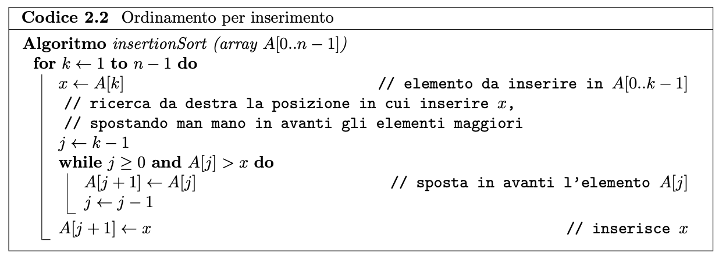
\includegraphics[scale=0.8]{insort}
\end{center}
InsertionSort è un algoritmo stabile, nel caso peggiore la complessità di tempo è $\Theta(n^2)$ ma nel caso migliore il numero di confronti da fare è $n-1$
\item BubbleSort\\
Scansiona l'array e confronto coppie adiacenti ripetutamente, scambio gli elementi se sono in ordine diverso. Alla fine dell'ultimo round l'elemento più grande finisce sul fondo.
\begin{center}
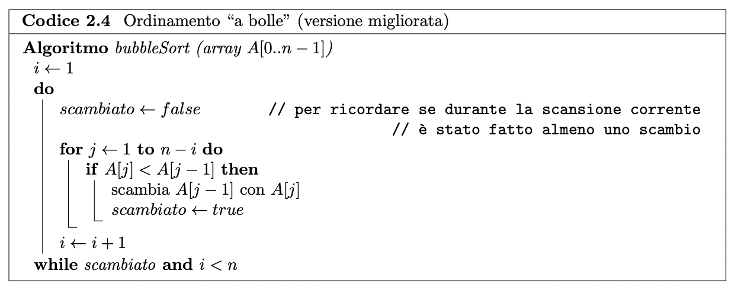
\includegraphics[scale=0.8]{bubsort}
\end{center}
BubbleSort è un algoritmo stabile, nel caso peggiore la complessità di tempo è $\Theta(n^2)$ ma nel caso migliore il numero di confronti da fare è $n-1$
\end{itemize}
\subsection{Algoritmi avanzati}
In particolare gli algoritmi avanzati sono MergeSort, QuickSort, HeapSort, sono algoritmi che utilizzano $\Theta(nlogn)$ confronti.
\begin{itemize}
\item MergeSort\\
Dividi l'array in porzioni unitarie, ordina ordina ricorsivamente le porzioni adiacenti fino a ricostruire l'array ordinato. 
\begin{center}
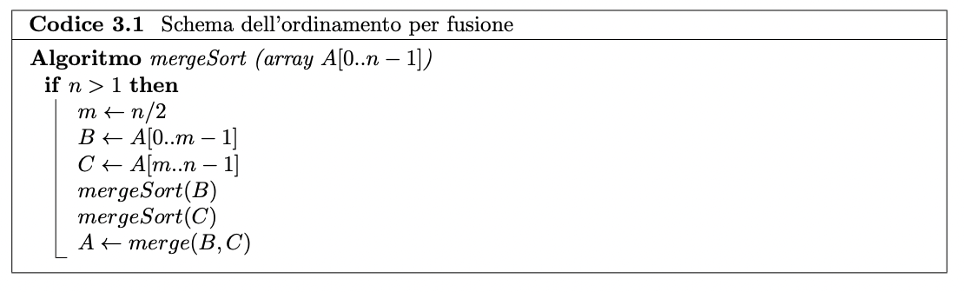
\includegraphics[scale=0.8]{mergsort}
\end{center}
MergeSort è un algoritmo stabile, non opera sul posto ed è più efficiente degli algoritmi visti in precedenza.\\ \\Per funzionare l'algoritmo MergeSort ha bisogno di un metodo che ci permetta di fare la fusione tra 2 array, in particolare dati due array $B, C$ dobbiamo avere un array $A$ che sia uguale all'unione tra $B, C$.\begin{center}
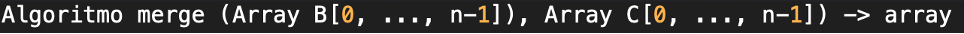
\includegraphics[scale=0.8]{merge}
\end{center}
\item QuickSort\\
1. Scegli un elemento n di A come perno\\
2. Inserisci tutti gli elementi $n \leq a$ in un array B\\
3. Inserisci tutti gli elementi $n > a$ in un array C\\
4. Ordina B e C\\
5. Unisci B e C
\begin{center}
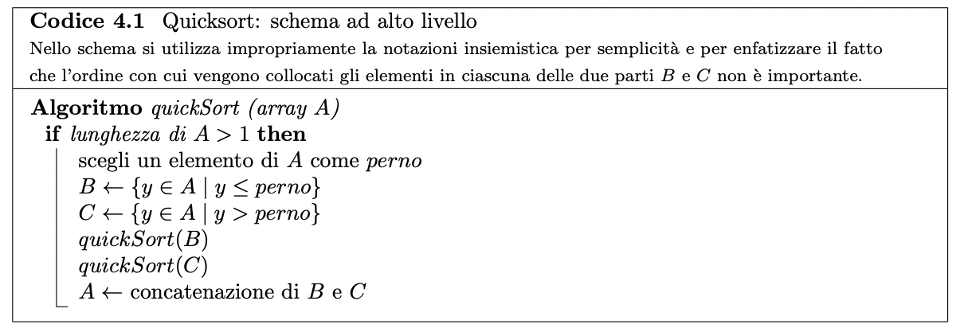
\includegraphics[scale=0.8]{quicksort}
\end{center}
QuickSort è il primo algoritmo instabile che incontriamo. Diversamente da MergeSort, QuickSort opera sul posto utilizzando due variabili aggiuntive. \\Nel caso ottimo l'algoritmo ha un tempo \begin{center} $T(n) = O(n * logn)$ \end{center}nel caso pessimo invece \begin{center} $T(n) = O(n^2)$ \end{center} Nel caso medio QuickSort opera in $T(n) = O(n * logn)$.
In media QuickSort è più efficiente di InsertionSort, SelectSort, BubbleSort e ha prestazioni peggiori di MergeSort solo nel caso peggiore. Da verifiche sperimentali possiamo concludere che QuickSort è l'algoritmo di ordinamento per array più efficiente. Possiamo inoltre concludere che in genere $T(n) = O(n * logn)$ è il tempo migliore possibile per gli algoritmi di ordinamento basati sul confronto
\end{itemize}
\section{Tecniche di risoluzione}
\subsection{Tecniche Divide-Et-Impera}
La tecnica del divide et impera è una tecnica di progettazione degli algoritmi suddivisibile in 3 fasi:
\begin{itemize}
\item dividere l'istanza dei dati in ingresso in più sottoinstanze disgiunte
\item risolvere ricorsivamente i problemi in ciascuna sottoistanza separatamente
\item combinare le soluzioni delle sottoinstanze per ricavare la soluzione dell'istanza iniziale.
\end{itemize}
L'efficienza del metodo dipende dal metodo di decomposizione e ricomposizione delle soluzioni parziali. Questa tecnica adotta un approccio top-down, i principali esempi che vediamo noi sono MergeSort e QuickSort. Una generalizzazione della tecnica può essere la seguente:
\begin{center}
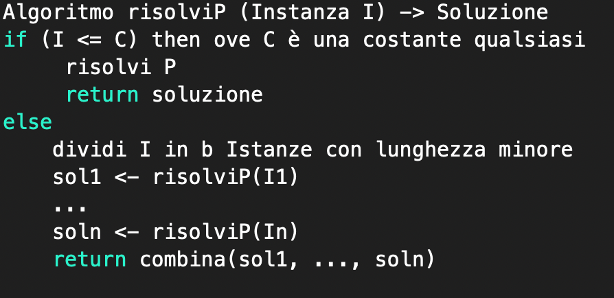
\includegraphics[scale=0.8]{divide}
\end{center}
Gli esempio che abbiamo visto durante il corso di applicazione di tecniche divide-et-impera sono:
\begin{itemize}
\item Algoritmo ricorsivo per calcolare il massimo ed il minimo subarray di un array di $n$ interi\\
L'array iniziale è suddiviso in 3 subarray disgiunti di $n/2$ interi, e ricorsivamente calcoliamo il massimo o il minimo di ciascun subarray.
\item Algoritmo di ricerca binaria in un array di $n$ interi\\
L'algoritmo divide l'array in due subarray di grandezza $n/2$ ricorsivamente, procedendo solo in uno dei due subarray.
\item Mergesort per array di $n$ elementi\\
L'algoritmo divide l'array in due subarray di grandezza $n/2$ ricorsivamente, e riordina ciascuno dei subarray, riunendoli alla fine
\item Quicksort per array di $n$ elementi\\
L'algoritmo divide l'array in tre subarray disgiunti composti rispettivamente dagli elementi $\leq$, $=$ e $\geq$. Il primo ed il terzo array sono riordinati ricorsivamente, e vengono poi concatenati i subarrays. 
\end{itemize}

\subsection{Dynamic Programming | Programmazione dinamica}
La programmazione dinamica è una tecnica di progettazione di algoritmi che diversametne dal divide-et-impera opera secondo una logica bottom-up; la risoluzione si basa sulla risoluzione di sottoproblemi progressivamente più grandi. Ne consegue che per tenere conto delle soluzioni ai sottoproblemi la tecnica di programmazione dinamica utilizza un'apposita tabella.\\
Possiamo dividere la tecnica di programmazione dinamica in quattro fasi:
\begin{itemize}
\item Identificazione dei sottoproblemi del problema iniziale
\item Predisporre una tabella ove memorizzare dinamicamente le soluzioni ai sottoproblemi a partire dai sottoproblemi più semplici, la cui soluzione è immediata
\item Si utilizzano le soluzioni dei sottoproblemi precedentemente risolti per risolvere sottoproblemi più difficili, con conseguente consultazione e aggiornamento della tabella
\item Si costruisce la soluzione finale a partire dalle soluzioni dei sottoproblemi risolti.
\end{itemize}
La programmazione dinamica, come negli algoritmi greedy, rappresentano problemi di ottimizzazione e seguono il principio di ottimalità, che garantisce che se una soluzione è ottima, anche le porzioni che vanno a comporre la situazione sono ottime
Gli esempio che abbiamo visto durante il corso di applicazione di tecniche programmazione dinamica sono:
\begin{itemize}
\item Allgoritmo di Floyd-Warshall per un grafo di $n$ vertici.
Identifica come sottoproblemi quelli di calcolare i percorsi più brevi tra tutte le coppie di vertici del grafo che passano per vertici di indice $\leq$ $k$ per ogni $1 \leq k$ $<$ $n$, predispone una tabella di $n + 1$ elementi (che sono delle matrici quadrate di ordine $n$) inizializzando il primo elemento in base alla matrice di adiacenza del grafo, avanza di un elemento alla volta determinandone il valore tramite una specifica formula applicata al valore dell’elemento precedente, e restituisce come risultato il valore dell’ultimo elemento. In pratica, non serve predisporre una tabella di matrici in quanto è sufficiente un’unica matrice per effettuare tutti i calcoli.
\item Algoritmo per la ricerca di un sottovettore di somma massima/minima\\
L'algoritmo lavorano creando due indici di supporto, che designano rispettivamente l'inizio e la fine del subarray che contiene il valore massimo. Viene creato un array $V$ di supporto che calcola i valori su cui effettuare le verifiche.
\begin{center}
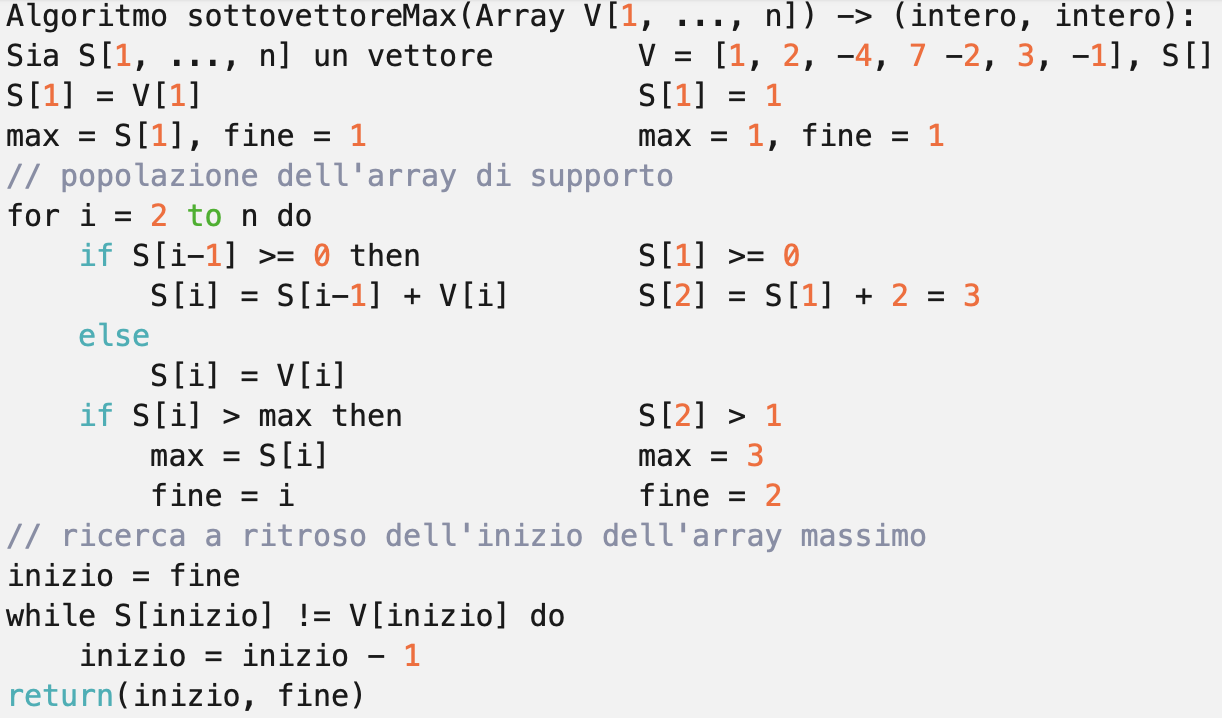
\includegraphics[scale=0.7]{sottomax}
\end{center}
Considero sottoproblemi $P(1), ... P(n)$ via via più difficili. Risolvo i sottoproblemi a partire dal più semplice $P(1)$, e da questi ricavo la soluzione di $P$. In questo caso $P(i)$ è trovare il sottovettore di somma massima che termina in posizione $i$. , mentre la soluzione di $P$ è la scelta tra le soluzioni di $P(1), ..., P(N)$ \\
Il tempo totale dell'algoritmo è dell'ordine di $T(n) = O(n)$
\item Algoritmo per la ricerca di un cammino di valore minimo su matrice\\
Data una matrice $n * n$ di interi determinare un cammino dalla prima all'ultima colonna di valore minimo minimo tale che \begin{enumerate}
\item l'inizio sia una posizione qualsiasi sulla prima colonna
\item per raggiungere la colonna successiva può muoversi sulla riga sopra, sulla stessa riga, o sulla riga sotto
\item la fine sia una posizione qualsiasi sull'ultima colonna
\end{enumerate}
Per impostare il problema con la programmazione dinamica identifichiamo: \begin{center}
- $P$: trovare il cammino di valore minimo in una matrice $n * n$\\
- $P(i, j)$: trovare il cammino di valore minimo che inizia nella colonna 1, e termina nella posizione $(i,j)$
\end{center}
La soluzione di $P$ si ricava dalle soluzioni di $P(1,n), P(2,n), ..., P(n,n)$. 
\subsection*{Matrice C dei risultati dei problemi P(i,j)}
Il valore $C[i,j]$ rappresenta il costo del cammino minimo che inizia nella posizione $1$, e termina nella posizione $(i,j)$, in particolare la sua formula è:
\begin{center}
$C[i,j] = M[i,j] + min\{C[i-1, j-1], C[i,j-1], C[i+1,j-1]\}$
\end{center}
Ovvero il valore della matrice iniziale sommata al valore minimo tra i valori raggiungibili.
\begin{center}
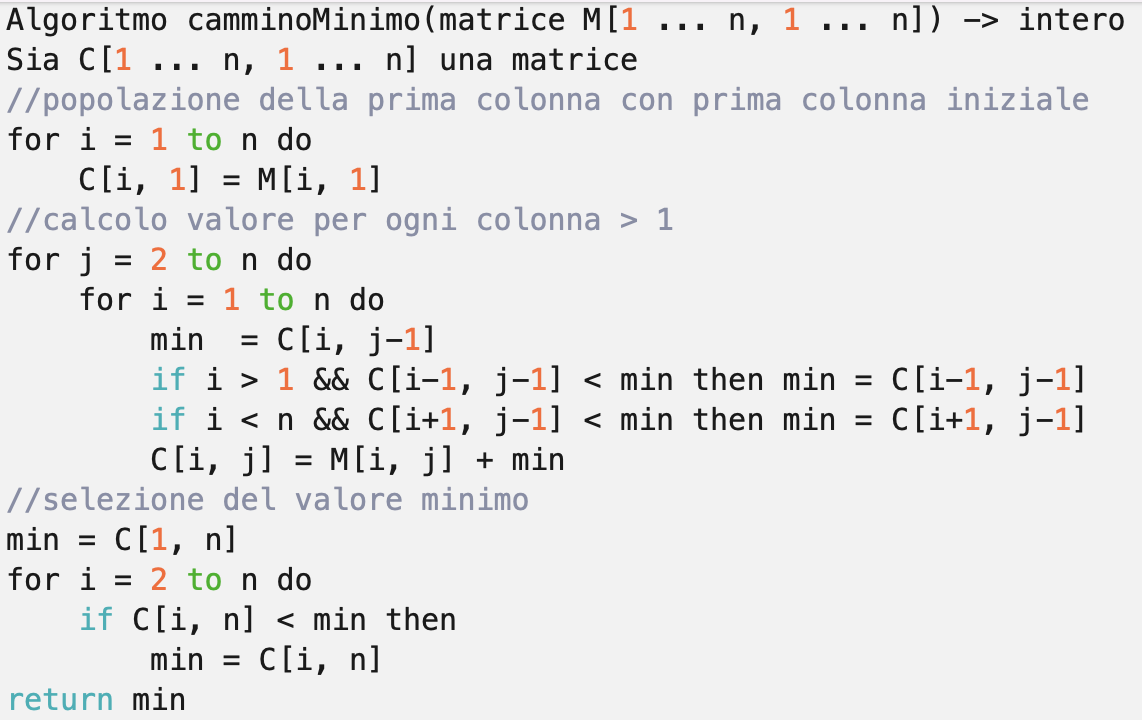
\includegraphics[scale=0.8]{cammmin}
\end{center}
Il tempo totale dell'algoritmo è dell'ordine di $T(n) = O(n^2)$
\end{itemize}








\subsection{Greedy Algorithms | Tecnica golosa}
La tecnica golosa si applica ai problemi di ottimizzazione in cui la soluzione è costruita scegliendo, ad ogni passo, l'elemento migliore nel momento. La soluzione che ricaviamo non è sempre la soluzione ottima, è tuttavia la soluzione più veloce da computare
Gli esempio che abbiamo visto durante il corso di applicazione di tecniche greedy sono:
\begin{itemize}
\item Algoritmo di Kruskal per grafo ricoprente minimo\\
L'algoritmo di Kruskal costruisce la soluzione considerando come candidati i singoli archi del grafo, scegliendo ad ogni passo l'arco di peso minimo tra i rimasti, ritenendo i singoli archi ammissibili se i vertici appartengono a due alberi diversi tra quelli costruiti fino a quel momento
\item Algoritmo di Prim per grafo ricoprente minimo\\
L'algoritmo di Prim costruisce la soluzione partendo da un grafo iniziale contenente un solo vertice $s$, considerando come candidati i rimanenti vertici del grafo scegliendo ad ogni passo quelli con distanza minima dall'albero libero costruito fino a quel momenti.
\item Algoritmo di Dijkstra per il calcolo di cammino minimo tra un vertice $s$ e tutti gli altri\\
L'algoritmo prende come soluzione iniziale un insieme vuoto (con input iniziale un vertice $s$), considerando come candidati i singoli vertici del grafo, scegliendo tra quelli rimasti quelli con distanza minima dal vertice sorgente.
\end{itemize}




\section{Tipi di dati}
Il tipo di una variabile rappresenta una variabile che stabilisce i valori che il dato può assumere e le operazioni che essa può svolgere. Le varie strutture dati che andiamo ad analizzare sono riconducibili a quattro classi fondamentali, ovvero: \emph{array, liste, alberi e grafi.} Le strutture dati possono essere caratterizzate dalla loro occupazione di memoria, che può essere statica, o dinamica.

\subsection{Dizionario | HashMap}
Il dizionario è una collezione di elementi ciascuno dei quali è caratterizzato da una \textbf{chiave}. Le operazioni che possiamo svolgere su un dizionario sono \emph{la ricerca, l'inserimento e la cancellazione} di un elemento. \\
Un dizionario può essere implementato utilizzando un array:\\
- se l'array è ordinato in base la chiave la ricerca ha costo $\Theta(logn)$ e l'inserimento costa $\Theta(n)$\\
- se l'array invece non è ordinato la ricerca costa $\Theta(n)$ e l'inserimento costa $\Theta(1)$\\\\
Un dizionario può essere anche implementato utilizzando collezioni, ovvero strutture statiche (con dimensione fissata all'inizializzazione), indicizzate ad esempio \emph{vectors e arraylists}; oppure utilizzando strutture collegate, dinamiche ad esempio \emph{liste e alberi}

\subsection{Liste concatenate}
Le liste concatenate sono un insieme di nodi collegati linearmente tra di loro. In particolare ogni nodo contiene:
\begin{itemize}
\item un dato della collezione
\item informazioni per accedere al prossimo nodo
\item informazioni per accedere al nodo precedente (nel caso delle doppiamente concatenate)
\end{itemize}
\begin{center}
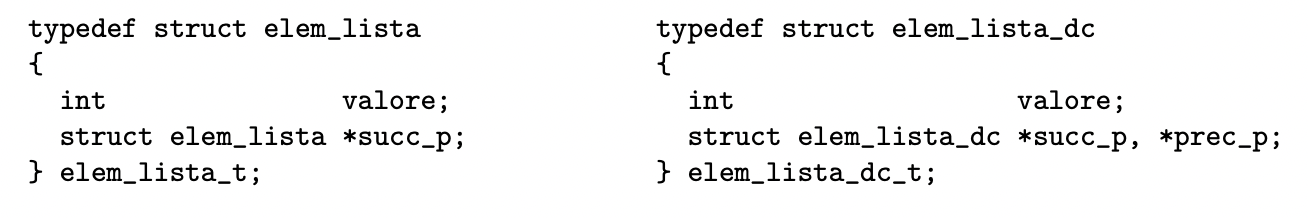
\includegraphics[scale=0.7]{conca}
\end{center}
I tipi di problemi che possiamo andare a svolgere sulle liste sono:
\begin{itemize}
\item problema della visita: data una lista attraversare tutti gli elementi una volta
\item problema della ricerca, data una lista ed un valore, stabilire se il valore è contenuto all'interno della lista, e l'indirizzo in caso affermativo
\item problema dell'inserimento, data una lista ed un valore, inserire il valore nella posizione appropriata
\item problema della rimozione, data una lista ed un valore, rimuovere il valore dalla lista
\end{itemize}

\subsection{Pila}
La pila, o stack, è una struttura dati che organizza i dati secondo una logica LIFO, il che significa che gli inserimenti e le rimozioni avvengono presso l'estremità della lista. Come in una lista la pila è individuata dall'indirizzo per primo elemento, chiamato cima. L'implementazione può avvenire con un array, o delle liste lineari. Le operazioni fondamentali che vengono svolte su una pila sono:
\begin{itemize}
\item isEmpty: che mi restituisce true se la pila è vuota, e false se la pila non lo è
\item push: dato un valore, lo aggiunge sulla pila
\item pop: dato un valore, lo rimuove dalla pila
\item peek: mi restituisce il valore in cima, senza modificarla
\end{itemize}

\subsection{Alberi con radice}
Gli alberi con radice (o solamenta albero) sono una struttura dati simile agli array, ma dotati di una rappresentazione gerarchica dei dati. I nodi possono essere definiti come padre, nodo interno, foglia e radice, mentre i collegamenti tra i nodi sono chiamati archi. In particolare quando parliamo di alberi possiamo identificare:
\begin{itemize}
\item la profondità come il numero massimo di nod da attraversare partendo dalla radice alla foglia più distante
\item grado di un nodo come il numero massimo di figli che un nodo può avere
\end{itemize}
I problemi classici che trattiamo per gli alberi sono: visita, ricerca, inserimento e rimozione. 
\subsubsection{Alberi binari}
Un albero è detto binario se ad ogni nodo sono associati al più 2 figli, chiamati rispettivamente figlio destro e figlio sinistro. 
\subsubsection{Alberi binari di ricerca}
Un albero è detto binario di ricerca se:
\begin{itemize}
\item tutti gli elementi nel sottoalbero sinistro hanno valore $<$ della chiave in $n$
\item tutti gli elementi nel sottoalbero destro hanno valore $\geq$ della chiave in $n$
\end{itemize}
Gli alberi binari di ricerca differiscono dagli alberi binari in quanto permettono una \emph{ricerca più efficiente} degli alberi binari. In particolare per ogni nodo incontrato si verifica se il valore si maggior o minore della chiave contenuta nel nodo. \\
L'inserimento e la rimozione devono invece garantire che l'albero binario risultante sia ancora un albero binario di ricerca.\\ La complessità degli algoritmi di ricerca, inserimento e rimozione con $n$ il numero di nodi, e $h$ la sua altezza:
\begin{center}
Caso ottimo: $T(n) = O(1)$\\
Caso pessimo: $T(n) = O(n)$\\
Caso medio: $T(n) = (log$ $n)$
\end{center}
\subsubsection{Alberi perfettamente bilanciati}
Un albero binario è detto perfettamente bilanciato se, per ogni nodo, il numero di nodi del suo sottoalbero sinistro, ed il numero di nodi del suo sottoalbero destro differiscono al più di 1.\\
\emph{Brutalmente: guardando sotto ogni sotto-nodo, la differenza tra il numero di nodi destro e sinistro è al massimo 1}\\
Siccome negli alberi perfettamente bilanciati, il bilanciamento dopo le operazioni di inserimento e rimozione sono costose sono stati introdotti una serie di alberi con forme di bilanciamento meno restrittive di quello perfetto.
\subsubsection{Alberi di ricerca AVL | Alberi bilanciati in altezza}
Un albero binario è detto bilanciato in altezza o AVL se, per ogni nodo, l'altezza del suo sottoalbero sinistro e l'altezza del suo sottoalbero destro differiscono al più di 1. Si noti che un albero perfettamente bilanciato anche bilanciato.
Gli alberi AVL sono particolari in quanto hanno un tempo di ricerca, inserimento e cancellazione pari che lavorano a tempo logaritmico:
\begin{center}
Per ricerca, inserimento e cancellazione:\\
$T(n) = O(log$ $n)$
\end{center}
\subsubsection{Alberi binario di ricerca rosso-nero}
Un albero binario di ricerca è detto rosso-nero se, dopo aver aggiunto un nodo sentinella come figlio di tutte le foglie, e dopo aver colorato ogni nodo di rosso o nero si ha che:
\begin{enumerate}
\item La radice è nera
\item La sentinella è nera
\item Se un nodo è rosso, tutti i suoi figli sono neri
\item per ogni nodo, tutti i percorsi dal nodo alla sentinella attraversano lo stesso numero di nodi neri
\end{enumerate}
Un albero binario di ricerca rosso-nero è una buona approssimazione di un albero binario di ricerca perfettamente bilanciato. 
\begin{center}
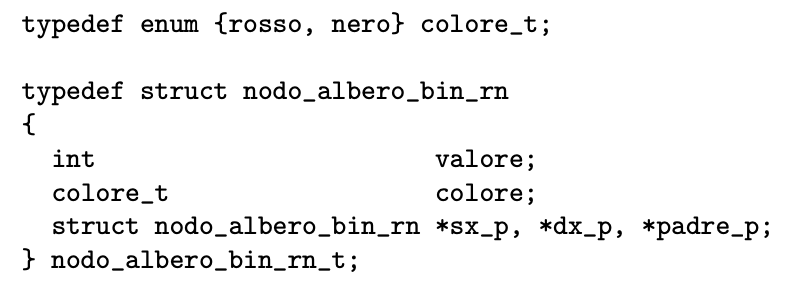
\includegraphics[scale=0.8]{rossonero}
\end{center}
\subsubsection{Alberi 2-3}
Un albero è detto 2-3 se ogni nodo interni ha 2-3 figli, e le foglie sono tutte allo stesso livello. I dati vengono inseriti all'interno delle foglie, mentre i nodi interni contengono solo informazioni di instradamento.\begin{itemize}
\item Se il nodo interno ha 1 valore, esso compare come sottofiglio sinistro, ed il sottofiglio destro è maggiore
\item Se il nodo interno ha 2 valori i sottofigli sono 3, i due valori compaiono come sottofiglio sinistro e centrale, mentre il sottofiglio destro è maggiore
\end{itemize}
\subsubsection{B-albero}
I B-alberi sono nati per rappresentare gli indici nelle basi di dati, l'obbiettivo è quello di minimizzare il numero di accessi. Le informazioni, a differenza degli alberi 2-3, sono presenti anche nei nodi interni.
Dato un b-albero di ordine $t$:
\begin{itemize}
\item i nodi interni hanno al massimo $2t$ figli
\item ogni nodo interno diverso dalla radice ha almeno $t$ figli
\item la radice ha almeno 2 figli
\item ogni foglia contiene $k$ chiavi ordinate
\end{itemize}
\begin{center}
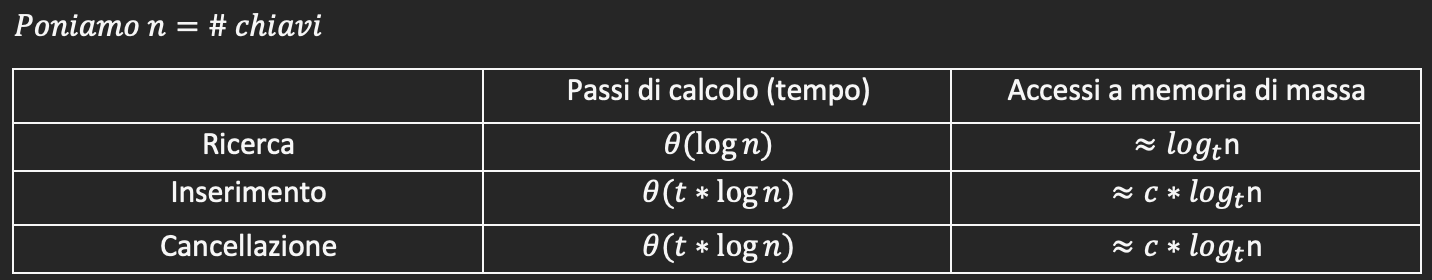
\includegraphics[scale=0.6]{balberi}
\end{center}
\subsubsection{Alberi binari quasi completi}
Un albero binario è detto \emph{quasi completo} quando è completo fino al penultimo livello e quindi tutte le foglie si trovano all'ultimo o penultimo livello.
\section{Heap}
Lo heap è un albero binario quasi completo, in cui la chiave contenuta in ciascun nodo è maggiore o uguale alle chiavi contenute nei figli. In particolare:
\begin{itemize}
\item tutte le foglie si trovano all'ultimo o penultimo livello
\item per ogni nodo, la chiave è $\geq$ delle chiavi contenute nei figli
\end{itemize}
\subsection*{Procedura risistema}
Consideriamo uno heap, se estraiamo un elemento è possibile sia necessario una \emph{risistemazione} dell'albero, in quanto potrebbe perdere la proprietà di heap. Questa procedura è implementata come segue:
\begin{center}
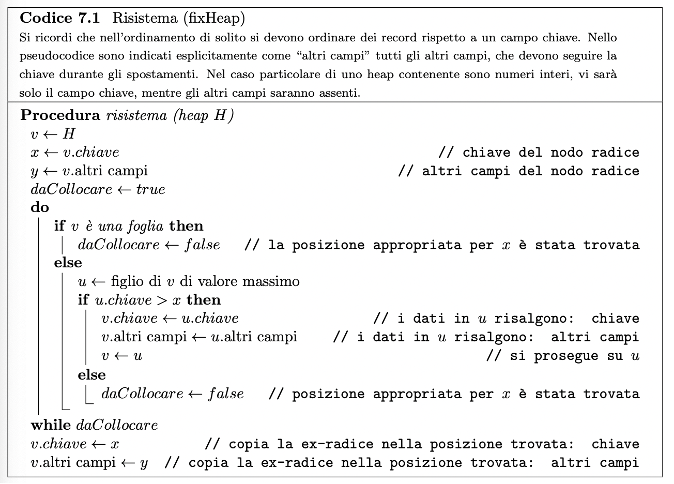
\includegraphics[scale=0.9]{risistemaheap}
\end{center}
\subsection*{Dato un albero binario quasi completo, come lo trasformo in uno heap?}
\begin{itemize}
\item con una tecnica divide-et-impera (top-down, ricorsiva)
\begin{center}
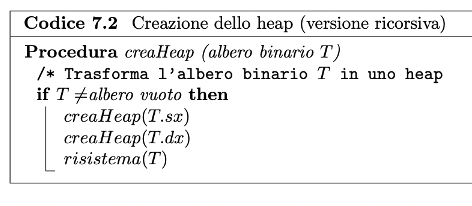
\includegraphics[scale=1]{creaheap1}
\end{center}
- se l'albero è vuoto, è già uno heap e non dobbiamo fare niente\\
- se l'albero non è vuoto, trasformo ricorsivamente in uno heap i due sottoalberi, e chiamo la procedura risistema, trasformando l'albero in uno heap
\item dai sottoalberi più piccoli a quelli più grandi (bottom-up, iterativa)
\begin{center}
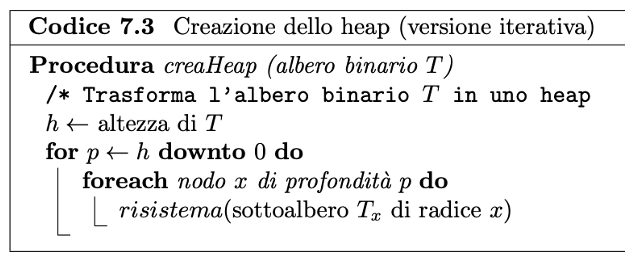
\includegraphics[scale=1]{creaheap2}
\end{center}
A partire dall'ultima foglia:\\
- considero ciascun nodo di profondità $h$ da destra a sinistra, trasformo in heap tutti i sottoalberi\\
- chiamo la procedura risistema\\
- ripeto sino ad arrivare alla radice
\end{itemize}
Abbiamo quindi tutti gli strumenti per finalmente implementare l'HeapSort

\section*{HeapSort}
HeapSort è un algoritmo iterativo basato sulla struttura dati chiamata heap. Questa struttura dati è rappresentabile con un array. L'heap è un albero binario quasi completo, in cui la chiave contenuta in ciascun nodo è maggiore o uguale al contenuto dei figli. Tutte le foglie si trovano all'ultimo o penultimo livello, e per ogni nodo, la chiave è $\geq$ delle chiavi nei figli.
\begin{center}
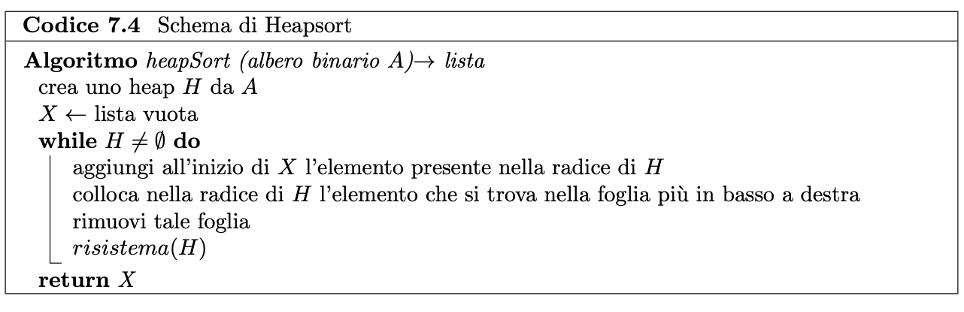
\includegraphics[scale=0.6]{heapsort}
\end{center}
Per funzionare l'HeapSort ha bisogno di una serie di metodi:\\
- risistema: che risistema un heap disordinato in un heap ordinato\\
- creaHeap: crea uno heap a partire da un albero binario\\\\
L'algoritmo di heapSort ha una complessità di \begin{center}
Per la \emph{parte esterna al while:} $T(n) = n$ \\
Per la \emph{parte interna al while:} $T(n) = nlogn$\\
Complessivamente: $O(nlogn)$
\end{center}
\section*{HeapSort basato su Arrays}
L'algoritmo HeapSort è basato su una struttura dati chiamata heap, per implementarlo tuttavia ci piacerebbe non dover utilizzare una struttura di supporto. Utilizziamo quindi l'array, predisponendo gli elementi all'interno nel seguente modo:
\begin{figure}[H]
\begin{center}
\begin{subfigure}[H]{0.5\linewidth}
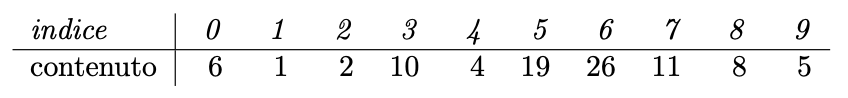
\includegraphics[width=\linewidth]{array}
\end{subfigure}
\begin{subfigure}[H]{0.5\linewidth}
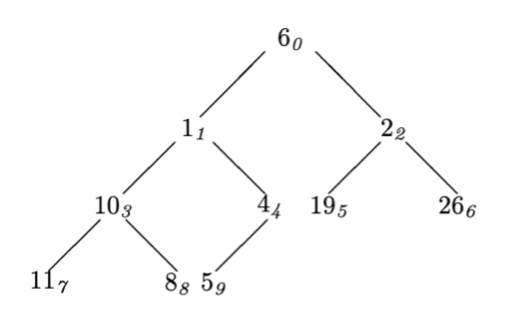
\includegraphics[width=\linewidth]{alberoo}
\end{subfigure}%
\end{center}
\end{figure}
Gli elementi dell'array sono inseriti da sinistra verso destra, garantendo che l'albero risultante sia sempre un albero binario quasi completo. L'elemento in posizione $0$ rappresenta la radice dell'array.
A questo punto possiamo implementare l'algoritmo \emph{HeapSort} direttamente sull'array, interpretandolo come un albero binario, senza l'utilizzo di puntatori.
\begin{center}
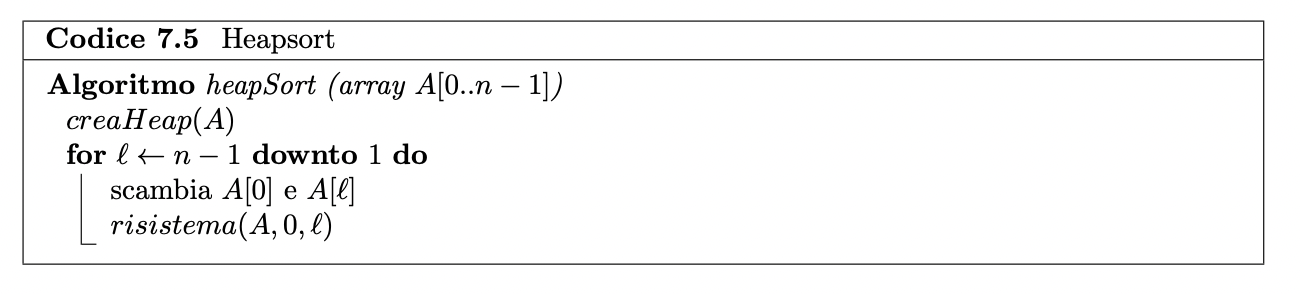
\includegraphics[scale=0.8]{heapar}
\end{center}
Nuovamente abbiamo bisogno di due metodi:\\
- risistema: che risistema l'array disordinato in uno heap\\
- creaHeap: utilizziamo la soluzione bottom-up, che trasforma in uno heap ogni sottoalbero a partire dall'ultima foglia
\subsection*{Considerazioni finali}
HeapSort è un algoritmo di ordinamento in loco, non stabile, che effettua $\theta(nlogn)$ confronti. Il tempo complessivo è  $\theta(nlogn)$

\section*{Una panoramica sugli algoritmi di ordinamento}
\begin{center}
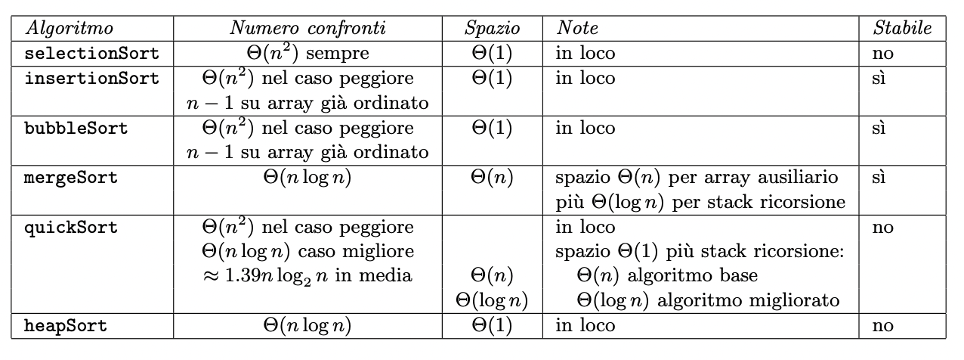
\includegraphics[scale=0.9]{riassunto}
\end{center}
\subsection*{Numero minimo di confronti}
Un qualsiasi algoritmo di ordinamento basato su confronti necessita, nel caso peggiore, un numero di confronti tra chiavi dell'ordine di $n log n$. A tale scopo osserviamo un confronto tra due chiavi $x_i$ e $x_j$, con risposta $si/no$. Per rappresentare la sequenza di decisioni percorribili per $n = 3$ elementi possiamo utilizzare un albero di decisione: 
\begin{center}
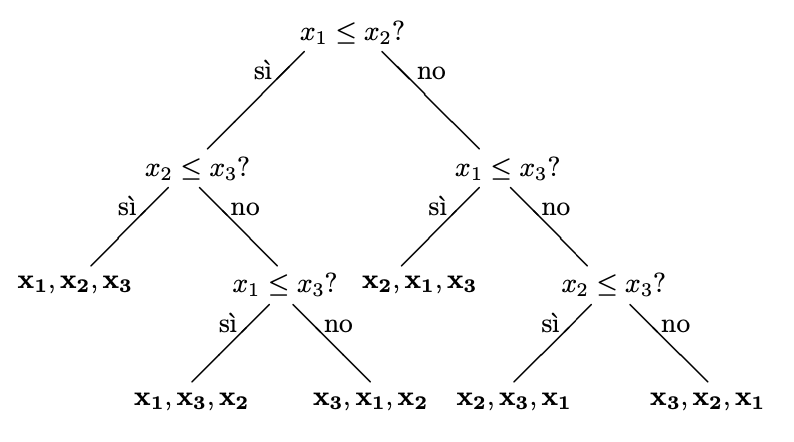
\includegraphics[scale=0.8]{albero}
\end{center}
Indipendentemente dal numero di confronti, l'albero avrà un numero di foglie uguale al numero di possibili ordini tra le chiavi, ovvero il numero di permutazioni di $n$, ovvero $n!$. \\Il numero massimo di confronti è pari alla profondità dell'albero, di nuovo $n=3$. Possiamo tuttavia verificare che la profondità dell'albero binario con $k$ foglie è almeno logaritmico in $k$.\\
Per trovare il numero di confronti necessari nel caso peggiore stimiamo la profondità minima che si ottiene da un albero con $n!$ foglie, calcolando il logaritmo di $n!$. Utilizziamo l'approssimazione di Stirling:
\begin{center}
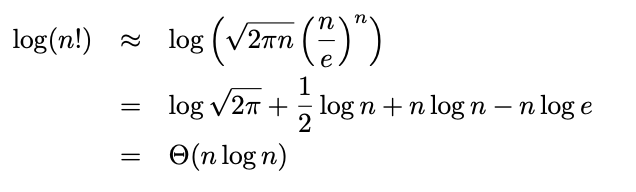
\includegraphics[scale=0.8]{stirling}
\end{center}
Concludiamo che un \emph{qualsiasi} algoritmo di ordinamento basato su confronti richiede al minimo un numero di confronti tra chiavi dell'ordine di $n log n$ per ordinare $n$ elementi.

\section*{Heap e Code con priorità}
Gli heap hanno altre applicazioni oltre all'utilizzo nell'algoritmo HeapSort, in particolare servono ad implementare le code con priorità. Le code con priorità sono strutture dati utilizzati in molti algoritmi, innanzitutto estendiamo le operazioni sugli heap:
\begin{itemize}
\item \emph{findMax | trova l'elemento di chiave massima}\\
L'elemento si trova in radice, l'operazione viene svolta in $O(1)$
\item \emph{deleteMax | cancella l'elemento di chiave massima}\\
Sostituiamo l'elemento in radice, con la foglia più a destra all'ultimo livello, per poi applicare $risistema$. Il numero di passi è proporzionale all'altezza dell'heap quindi $O(logn)$
\item \emph{insert | inserisci un nuovo elemento}\\
L'inserimento avviene con l'aggiunta alla prima posizione libera più a sinsitra dell'ultimo livello, o come prima foglia ad un nuovo livello. Non possiamo utilizzare la funzione $risistema$, ma dobbiamo utilizzare un approccio dal basso, con $risistemaDalBasso$. Il numero di passi è proporzionale all'altezza dell'heap quindi $O(logn)$
\item \emph{delete | cancella un elemento}\\
Per cancellare un elemento lo sostituiamo con la foglia più a destra dell'ultimo livello, che viene rimossa, e risistemiamo l'heap. Sia $x$ la chiave del nodo n da cancellare, e $f$ la chiave della foglia più a destra dell'ultimo livello:\\
- se $f < x$ utilizziamo $risistema$\\
- se $f > x$ utilizziamo $risistemaDalBasso$\\
In entrambi i casi il numero di passi è pari a $O(logn)$
\item \emph{changeKey | modifica la chiave di un elemento}\\
Modifica la chiave associata ad un nodo $n$, se:\\
- la chiave viene diminuita, utilizziamo $risistema$\\
- la chiave viene aumentata, utilizziamo $risistemaDalBasso$
\end{itemize} 
\subsection*{Code con priorità}
Utilizzando gli heap e le operazioni descritte possiamo implementare strutture a coda, in cui gli elementi vengono estratti secondo un criterio di priorità. In particolare le operazioni di una coda con priorità sono:
\begin{itemize}
\item \emph{findMin() | restituisce l'elemento minimo della coda}
\item \emph{deleteMin () | rimuovere l'elemento minimo della coda}
\item \emph{insert(e, k) | inserisce nella coda un elemento e associa una chiave}
\item \emph{delete(e) | rimuove l'elemento}
\item \emph{changeKey(e, d) | modifica la priorità dell'elemento}
\end{itemize}

\section*{Algoritmi di ordinamento non basati su confronti}
\subsection*{IntegerSort}
E' il primo algoritmo di ordinamento non basato su confronti. Oltre all'array da ordinare dobbiamo fornire anche un intero che rappresenti il range degli elementi all'interno dell'array. Viene creato un array ausiliario di contatori, che conta le occorrenze all'interno all'array $A$.\\ Infine viene riempito $A$ con i valori ordinati. 
\begin{center}
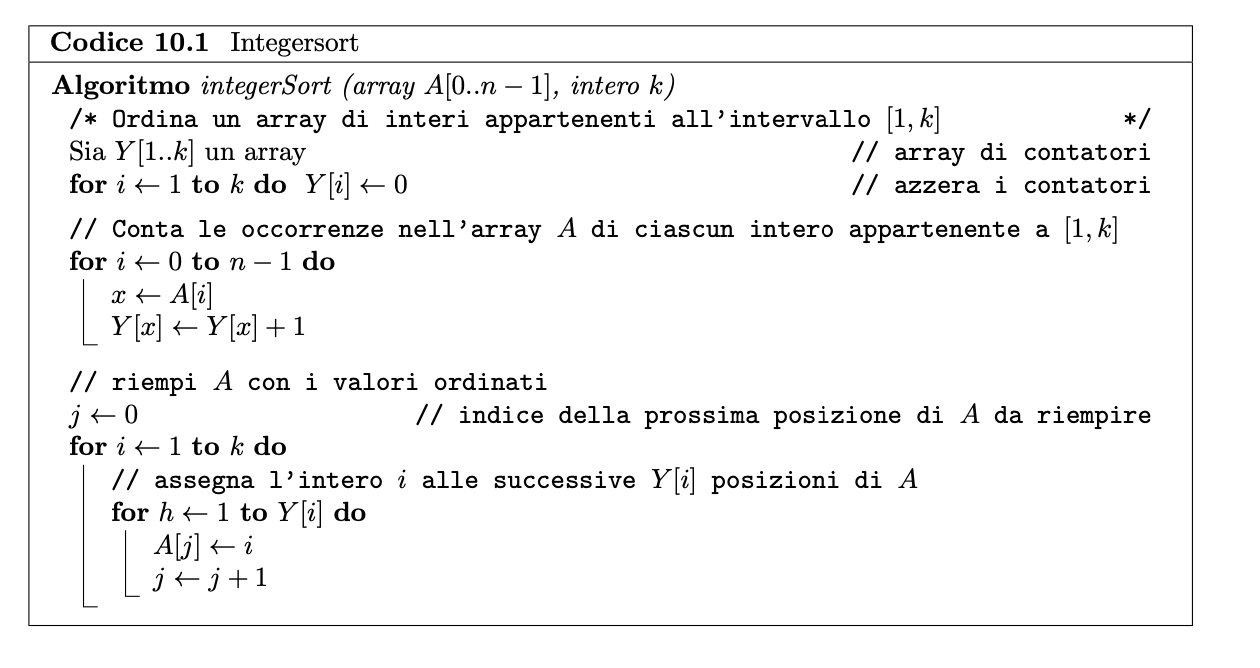
\includegraphics[scale=0.7]{integer}
\end{center}
\subsection*{BucketSort}
E' il secondo algoritmo di ordinamento non basato su confornti che incontriamo, ed utilizza le code. Nuovamente oltre all'array l'algoritmo necessita del range dell'array $A$. 
\begin{center}
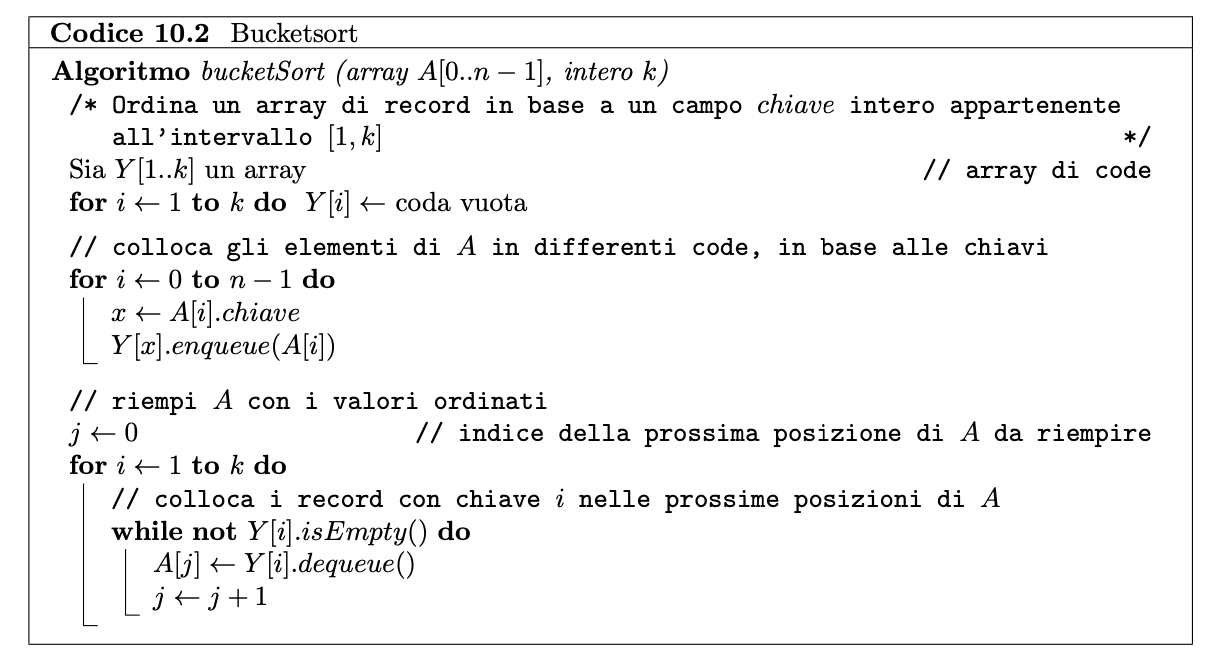
\includegraphics[scale=0.7]{bucket}
\end{center}
Vengono create una serie di code per ogni $n < k$, che vengono popolate con gli elementi presenti nell'array $A$. Il BucketSort è un algoritmo stabile, principalmente utilizzato per riordinare liste, manipolando direttamente i puntatori.
\subsection*{RadixSort}
Consideriamo di dover ordinare una serie di dati con chiavi intere. Possiamo applicare BucketSort prima sulle unità, poi decine, poi centinaia e così via. L'algoritmo riordina a partire dal \emph{least significant digit}. 
 \begin{center}
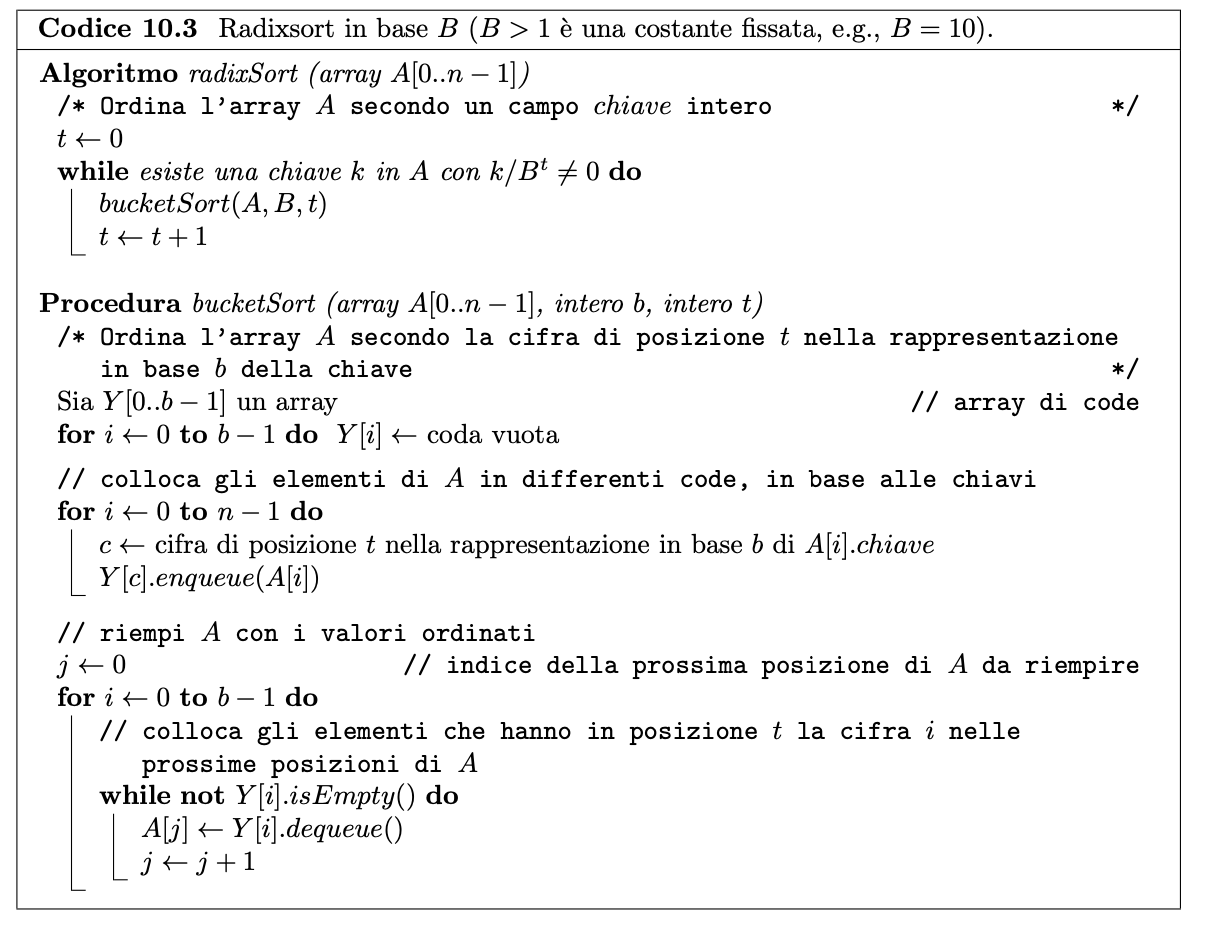
\includegraphics[scale=0.7]{radix}
\end{center}

\section*{Tecniche Union-Find}
Gli algoritmi \emph{union-find} lavorano su partizioni, e prendono il nome dalle due operazioni più svolte. Supponiamo quindi di avere una collezione $S$ di $n$ elementi distinti:
\begin{itemize}
\item Union(A, B): unisce gli insieme A, B in un unico insieme, il nuovo nome dell'insieme è A
\item Find(x): dato un elemento, restituisce il nome dell'insiemi che lo contiene
\item MakeSet(x): dato un elemento, crea un nuovo insieme con nome $x:{x}$
\end{itemize}
Vi sono vari tipi di soluzioni utilizzati, divisibili in soluzioni elementari, e soluzioni evolute.
In tutte le soluzioni presentate ogni insieme è rappresentato da un albero con radice in cui:
\begin{itemize}
\item i nodi rappresentano gli elementi dell'insieme
\item le radici rappresentano i nodi dell'insieme
\end{itemize}
I puntatori puntano verso l'alto, ed una partizione rappresenta una foresta di alberi.

\subsection*{Algoritmi QuickFind}
Negli algoritmi QuickFind gli elementi dell'insieme rappresentano le foglie, mentre i nomi dell'insieme rappresentano la radice. Ricordiamo che i puntatori puntano verso l'alto.
\begin{itemize}
\item Union(A, B): spostiamo i puntatori che puntavano da $B$, ad $A$\\
Questa operazione lavora in tempo $T(n) = O(n)$
\item Find(x): restituiamo l'elemento in tempo $T(n) = O(1)$
\item MakeSet(x): crea un nuovo albero, con foglia e radice uguale, in tempo $T(n) = O(1)$
\end{itemize}
Possiamo migliorare gli algoritmi con il \emph{QuickFind con bilanciamento}.
In particolare notiamo che nell'operazione di \textbf{Union(A,B)}, se $B$ ha più elementi di $A$, anziché collegare gli elementi di $B$ ad $A$, ci conviene collegare gli elementi di $A$ sotto $B$, e rinominare la radice. Miglioriamo l'efficienza, e al massimo dobbiamo spostare $n/2$ puntatori. Il tempo rimane dell'ordine di $T(n) = O(n)$ 

\subsection*{Algoritmi QuickUnion}
Negli algoritmi QuickUnion gli elementi dell'insieme sono rappresentati dai nodi, mentre l'elemento che da il nome all'insieme è la radice. Gli alberi sono di varia altezza. La differenza con gli alberi QuickFind è che consentiamo agli alberi di avere altezza maggiore di 1.
\begin{itemize}
\item Union(A, B): spostiamo il puntatore di $B$, ad $A$
Questa operazione lavora in tempo $T(n) = O(n)$
\item Find(x): restituiamo l'elemento in tempo $T(n) = O(n)$, dato che dobbiamo risalire da $x$ fino alla radice
\item MakeSet(x): crea un nuovo albero, con foglia e radice uguale, in tempo $T(n) = O(1)$
\end{itemize}
Nuovamente consideriamo un'operazione di \textbf{Union(A,B)}, possiamo migliorare l'efficienza, attaccando la radice dell'albero più basso sotto a quella dell'albero più alto. Chiamiamo questa $union$ migliorata \emph{QuickUnion by rank}

\section*{Grafi}
 Si dice grafo diretto o orientato una coppia $G = (V,E)$ ove $V$ è un insieme di vertice o nodi ed $E$ è una relazione binaria su $V$
 \begin{itemize}
\item I grafi possono essere non orientati/simmetrici, ovvero con archi senza freccia; oppure orientati/diretti, ovvero gli archi hanno frecce.
\item un cammino da $x$ a $y$ è una sequenza di vertici che porti da $x$ a $y$, in particolare un cammino è detto semplice se non contiene vertici ripetuti. Un ciclo è un cammino da vertice $x$ a $x$ 
\item un ciclo semplice è un ciclo in cui è ripetuto solo il vertice iniziale, alla fine 
\item una catena tra $x$ e $y$ è una sequenza di nodi collegati da archi orientati, ma di cui si ignora l’orientamento. Un circuito è una catena chiusa
\item un sottografo è un grafo, formato da un sottoinsieme di vertici e archi del grafo iniziale
\item un cammino Euleriamo è un cammino che attraversa ogni arco del grafo una sola volta (è quindi un ciclo)
\item un cammino Hamiltoniano è un cammino che attraversa ogni vertice una sola volta
\end{itemize}

\subsection*{Alberi e foreste}
Un albero è un grafo non orientato, connesso e privo di cicli. Una foresta è un insieme di alberi.\\
Un albero di supporto o ricoprimento (spamming tree) è un albero con gli stessi vertici, ma con gli archi che sono un sottoinsieme del grafo iniziale; un qualunque sottografo che contiene lo stesso numero di vertici, e che gli archi sia un sottonisieme degli archi.\\
\subsection*{Rappresentazione dei grafi}
Consideriamo i seguenti grafi non orientati, ed orientati
\begin{center}
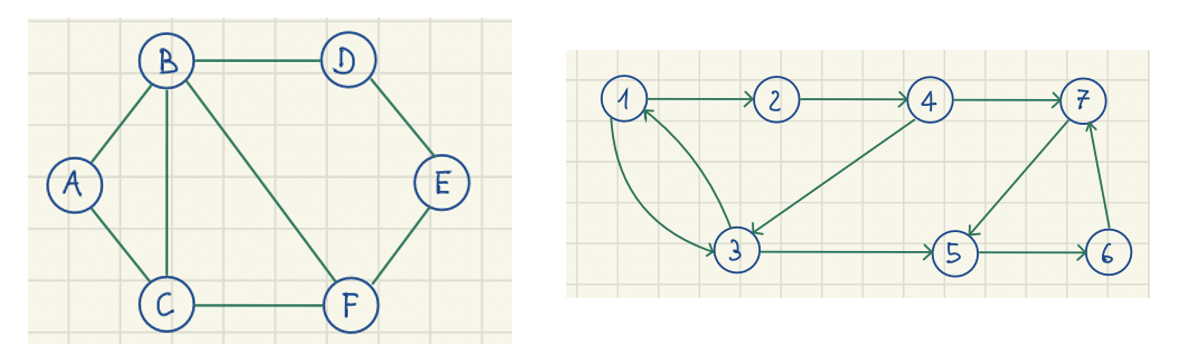
\includegraphics[scale=0.8]{b1}
\end{center}
Un grafo può essere rappresentato con
\begin{itemize}
\item Lista di archi\\
Una lista di archi è una struttura dati formata da 2 strutture, una lista che rappresenta i vertici, e una che rappresenta gli archi. Gli archi vengono rappresentati come un elenco che contiene le coppie di vertici, e gli archi che l'arco collega.
Questa rappresentazione è comoda per visualizzare i vertici di un arco, ma non per ricostruire la forma iniziale di un grafo. Lo spazio occupato è $O(m+n)$ ove $m$ è il numero di vertici, e $n$ il numero di archi
\item Lista di adiacenza\\
Una lista di adiacenza è una struttura dati formata da una lista primaria dei vertici e più liste secondarie degli archi.
La lista primaria contiene un elemento per ciascun vertice del grafo, il quale contiene a sua volta la testa della relativa lista secondaria. La lista secondaria associata ad un vertice descrive tutti gli archi uscenti da quel vertice, in quanto contiene gli indirizzi di tutti i vertici adiacenti al vertice in questione.
\begin{center}
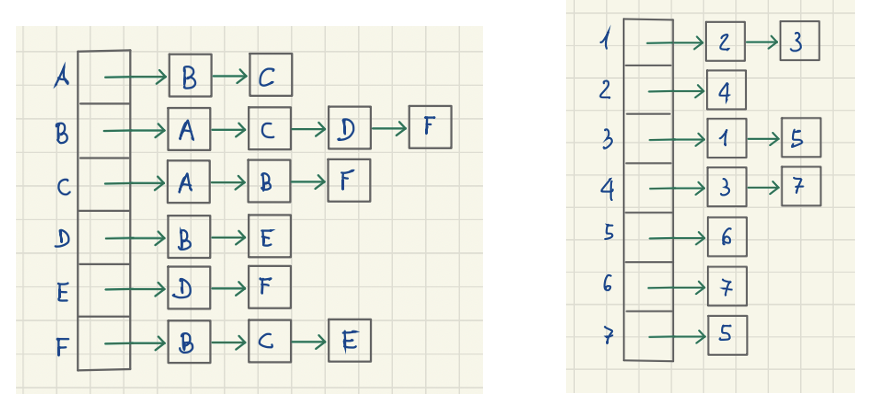
\includegraphics[scale=0.8]{b2}
\end{center}
L’accesso ad ognuno di essi necessita dell’indirizzo del primo elemento della lista primaria, l’accesso ad un vertice avviene scorrendo tutti i vertici che precedono il vertice in questione nella lista primaria.
\item Lista di incidenza\\
Una lista di incidenza è una struttura dati formata sostituendo la lista dei vertici delle liste di adiacenza, con liste di archi.
\begin{center}
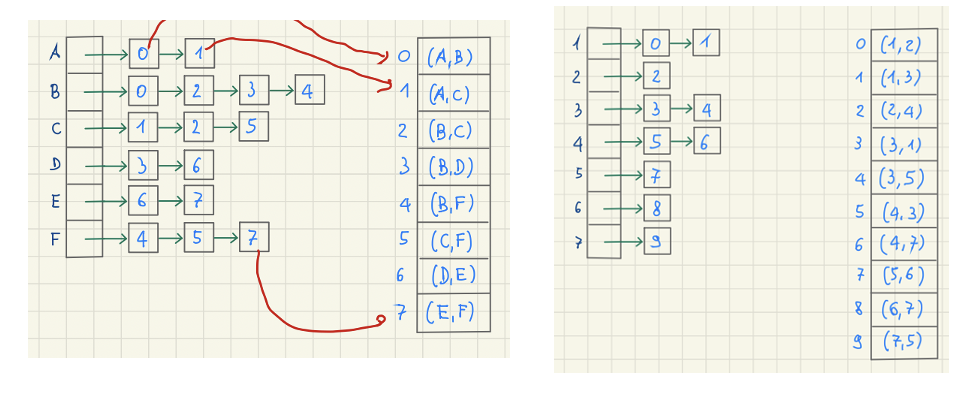
\includegraphics[scale=0.8]{b3}
\end{center}
Anche in questo caso lo spazio utilizzato è $O(m+n)$
\item Matrice di adiacenza\\
Una matrice di adiacenza creata a partire da un grafo $G$ è una matrice in cui il valore\begin{center}
$M(u,v) = 1$ sse $(u,v)\in E$
\end{center}
Se una matrice non è orientato, la matrice generato è una matrice simmetrica.
Lo spazio occupato da questa struttura è $O(n^2)$
\begin{center}
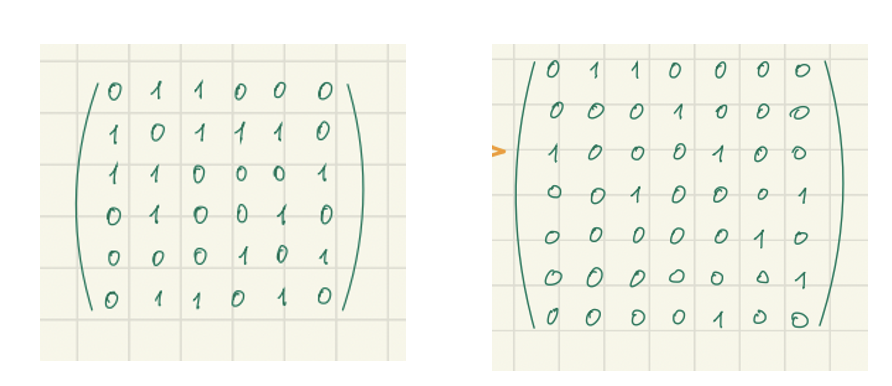
\includegraphics[scale=0.8]{b4}
\end{center}
\item Matrice di incidenza\\
Una matrice di incidenza creata a partire da un grafo $G$ è una matrice in cui:\\
- ogni riga rappresenta un vertice\\
- ogni colonna rappresenta un arco
\begin{center}
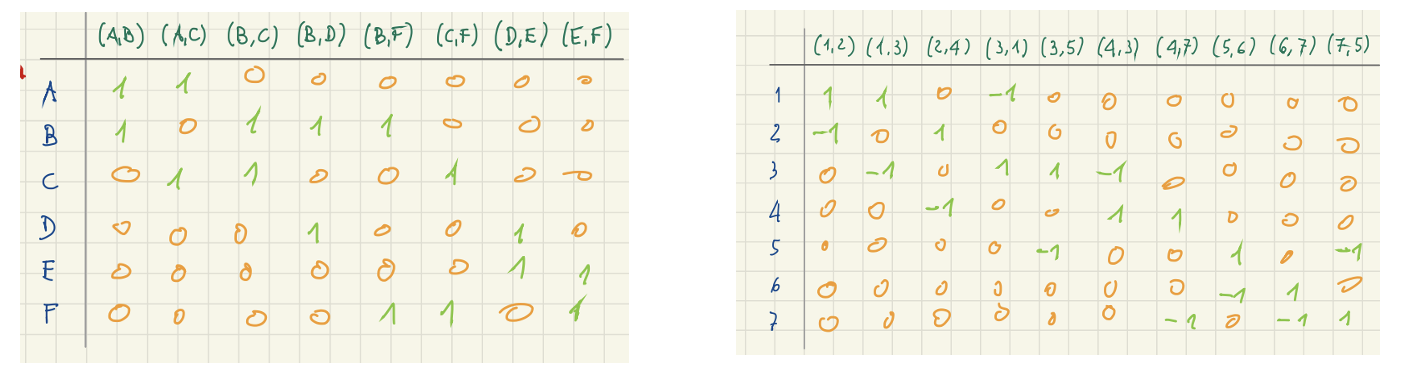
\includegraphics[scale=0.6]{b5}
\end{center}
Nel caso dei grafi orientati, il valore $M(u,v) = 1$ se l'arco è uscente, mentre è $M(u,v) = -1$ quando l'arco è entrante, $M(u,v) = 0$ quando non è incidente. Lo spazio occupato da questa struttura è $O(n*m)$
\end{itemize}

\section*{Attraversamento dei grafi}
Data la generalità della loro struttura, nel caso dei grafi ci sono ancora più alternative per effettuare una visita di quelle viste nel caso degli alberi binari. Di solito i vertici di un grafo $G = (V,E)$ vengono attraversati in maniera sistematica procedendo in ampiezza (breadth-first search) o in profondità (depth-first search).
\subsection*{Visita in ampiezza | Breadth-first Search}
La visita in ampiezza viene svolta nel seguente modo, a partire da un vertice $s$
\begin{itemize}
\item si visitano i vertici adiacenti ad $S$ aggiungendo man mano in una coda gli elementi
\item si visitano i vertici adiacenti ai vertici adiacenti ad $S$ che non sono ancora stati visitati.
\end{itemize}
\begin{center}
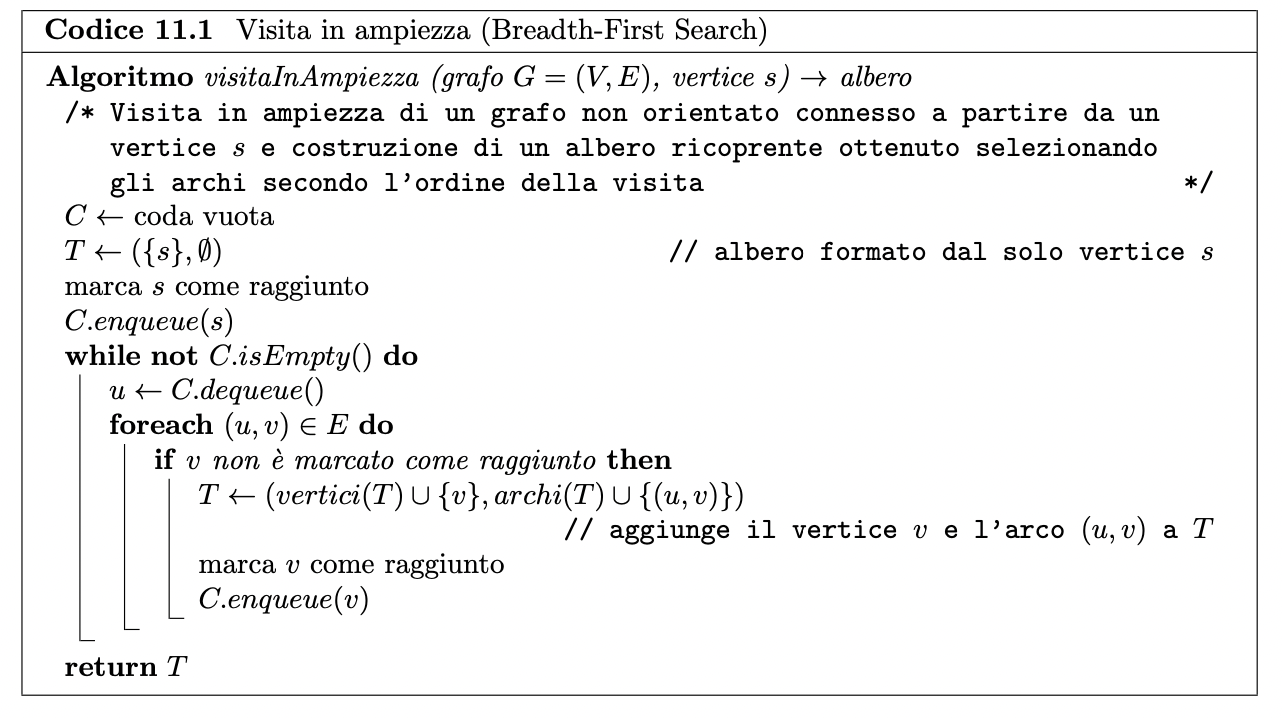
\includegraphics[scale=0.6]{ampiezza}
\end{center}

\subsection*{Visita in profondità | Depth-first Search}
La visita in ampiezza viene svolta ricorsivamente, a partire da un vertice $s$
\begin{itemize}
\item si visitano i vertici non ancora visti, fermandoci ad un vertice privo di vicini non ancora visitati
\item si ripete dal passo precedente, partendo dall'ultimo vertice sul cammino precedente che ha un vertice non raggiunto
\end{itemize}
\footnotesize{si parte da un vertice, e cerchiamo di esplorare il più possibile fino a quando non posso più muovermi. A quel punto torno indietro fino a quando non trovo una strada che posso percorrere.}
\begin{center}
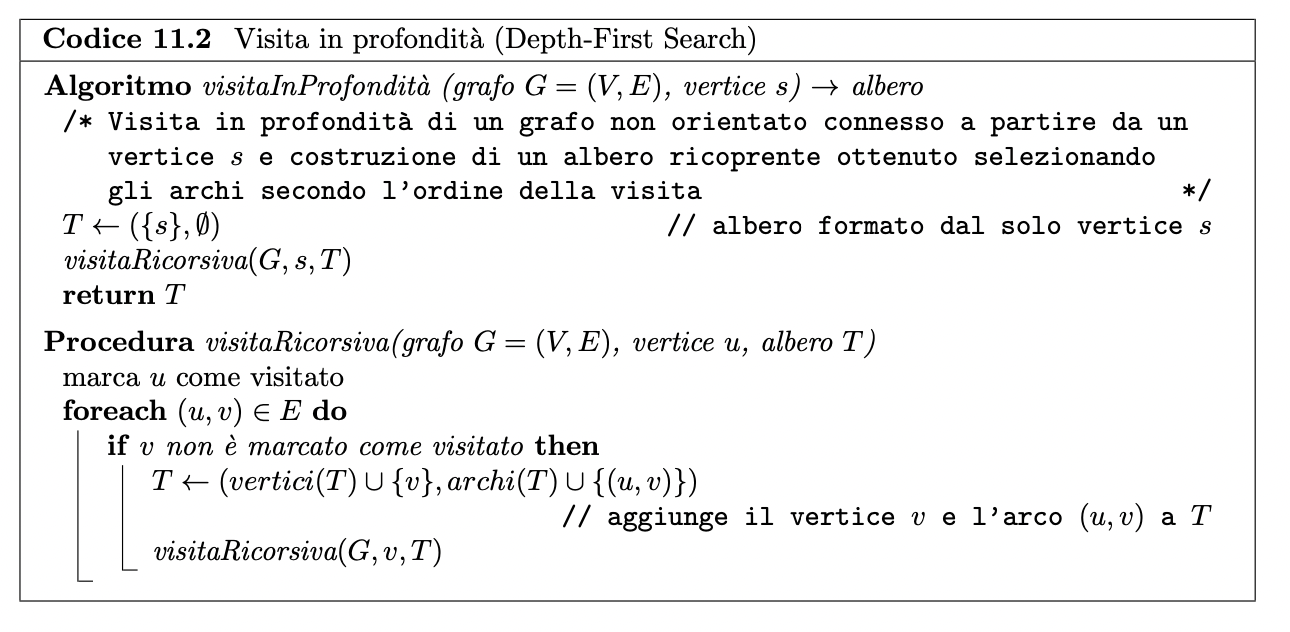
\includegraphics[scale=0.6]{profo}
\end{center}

\section*{Problemi di ottimizzazione e algoritmi Greedy}
Dato un problema $P$ di ottimizzazione:\begin{itemize}
\item C l'insieme di soluzioni candidati
\item Trovare $S \in C $ soluzione ottima
\end{itemize}
La tecnica golosa si applica ai problemi di ottimizzazione in cui la soluzione è costruita scegliendo, ad ogni passo, l'elemento migliore nel momento. La soluzione che ricaviamo non è sempre la soluzione ottima, è tuttavia la soluzione più veloce da computare.

\section*{Grafo pesato}
Consideriamo un grafo $G = (V, E)$, associamo una funzione $\omega : E \rightarrow R$ chiamata funzione peso.\begin{center}
Grafo pesato: $G = (V, E,\omega)$\end{center}
Dato un grafo pesato possiamo analizzare una serie di problemi:
\begin{itemize}
\item problema dei cammini minimi
\item problema degli alberi ricoprenti minimi (su grafi non orientati)
\end{itemize}
\begin{center}
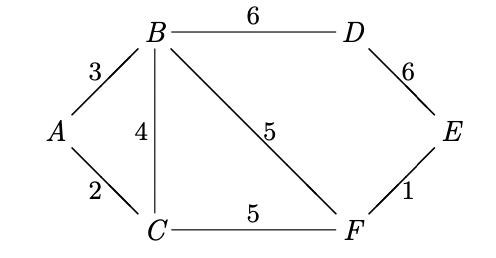
\includegraphics[scale=0.6]{grafopesato}
\end{center}

\subsection*{Albero ricoprente minimo}
Sia  $G = (V, E,\omega)$ un grafo pesato, trovare l'albero ricoprente minimo tra i possibili. Introduciamo quindi due algoritmi per trovare gli alberi ricopenti minimi di grafo connessi, non orientati e pesati, chiamati \emph{algoritmo di Kruskal}, e \emph{algoritmo di Prim}, entrambi basati sulla strategia greedy
\subsection*{Algoritmo di Kruskal}
L'algoritmo di Kruskal risolve il problema costruendo un grafo $T$ che ha gli stessi vertici di $G$ e, inizialmente, è privo di archi. \\
- L’algoritmo esamina gli archi di $G$ in ordine di peso non decrescente. \\
- Un arco viene aggiunto a $T$ se, insieme a quelli già scelti, non forma cicli, altrimenti viene scartato e non sarà più considerato. \\
- Ogni volta che si aggiunge un grafo, si connettono tra loro due alberi della foresta che diventano, con l’arco aggiunto, un unico albero. \\
- Alla fine, quando sono stati esaminati tutti gli archi, $T$ contiene un unico albero che è un albero ricoprente di peso minimo per il grafo G dato.
\begin{center}
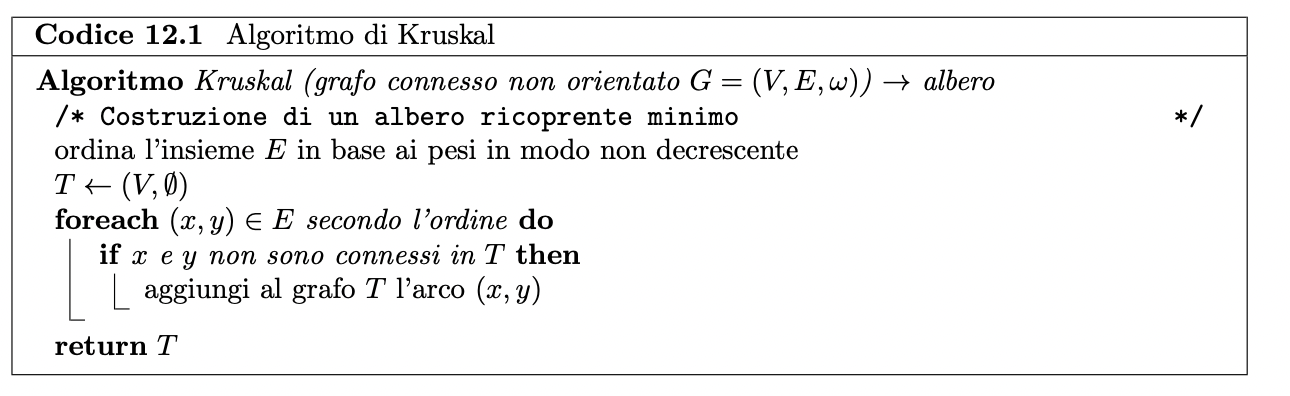
\includegraphics[scale=0.7]{kruskal}
\end{center}
L'algoritmo di Kruskal è implementabile attraverso lo union-find, con tempo totale $O(mlog^*m)$

\subsection*{Algoritmo di Prim}
Dato in ingresso un grafo connesso, non orientato con pesi sugli archi, l’algoritmo inizia costruendo un albero $T$ formato da un unico vertice $s$ qualsiasi del grafo. \\
Ad ogni passo, l’albero $T$ viene espanso scegliendo, tra tutti gli archi che hanno un vertice in $T$ e l’altro non in $T$, un arco di peso minimo. Tale arco viene aggiunto a $T$ (insieme al vertice che non era in T).\\
L’algoritmo di Prim può essere implementato ricorrendo a una coda con priorità $C$, contenente un elemento per ogni vertice che deve essere ancora inserito nell’albero.
\begin{center}
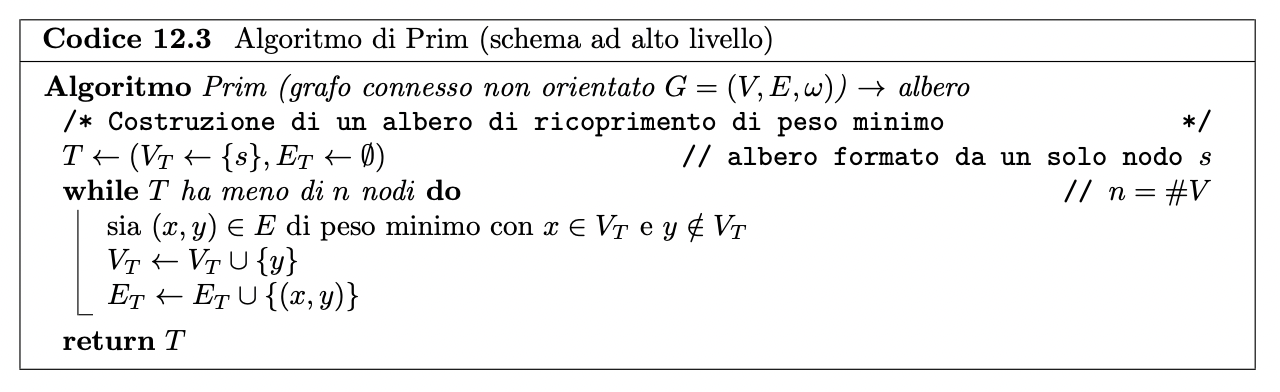
\includegraphics[scale=0.7]{prim}
\end{center}
L'algoritmo di Prim è implementabile con liste di adiacenza o incidenza, con code di priorità, e con code di priorità.
Per l'analisi del tempo supponiamo che il grafo in ingresso sia rappresentato mediante una lista di adiacenza o incidenza. Il tempo totale è $O(m log n)$


\section*{Problema dei cammini minimi}
Consideriamo $G = (V, E,\omega)$ un grafo pesato orientato, il problema dei cammini minimi ci chiede di trovare un cammino, tra i cammini possibili, che sia il minimo possibile. In particolare \begin{itemize}
\item se tutti i pesi sono positivi, allora il cammino è uno semplice
\item se ci sono pesi negativi, ma non cicli negativi, allora tra una coppia di vertici esiste un cammino minimo semplice.
\end{itemize}
Per rappresentare i grafi pesati, come avevamo visto in precedenza, utilizziamo matrici dei pesi, e liste di adiacenza.
I problemi che possiamo trovare sui cammini minimi sono:
\begin{enumerate}
\item trovare il cammino minimo tra 2 vertici \\
Non esiste un algoritmo diretto, ma possiamo applicare Dijkstra per risolverlo 
\item trovare i cammini minimi tra un vertice S e tutti gli altri\\
- Applicare Dijkstra se non ci sono pesi negativi, con tempo $T(n) = O(m + nlongn)$\\
- Applicare Bellman Ford, anche con pesi negativi, con tempo $T(n) = O(m*n)$
\item trovare i cammini minimi tra ogni coppia di vertici\\
- Applicare Floyd-Warshall, anche con pesi negativi, con tempo $T(n) = O(n^3)$
\end{enumerate}

\subsection*{Algoritmo di Floyd \& Warshall}
L'algoritmo di Floyd \& Warshall risolve il problema di cammino minimo tra due vertici attraverso una rappresentazione del grafo a matrice di adiacenza, basato sulla strategia della programmazione dinamica. Sia\begin{itemize}
\item $V = {v_1, ..., v_n}$ l'insieme dei vertici numerati
\item $d_{ij}$ il peso del cammino minimo tra $v_i$ e $v_j$
\end{itemize}
Viene impostata una matrice delle distanze $D$, con valore $d^{k}_{ij}$, che cambia per $k=0$ e $k > 0$
\begin{center}
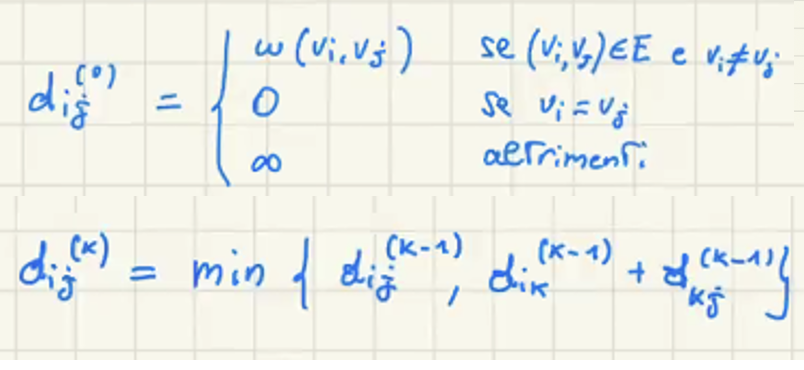
\includegraphics[scale=0.5]{floyd2}
\end{center}\begin{center}
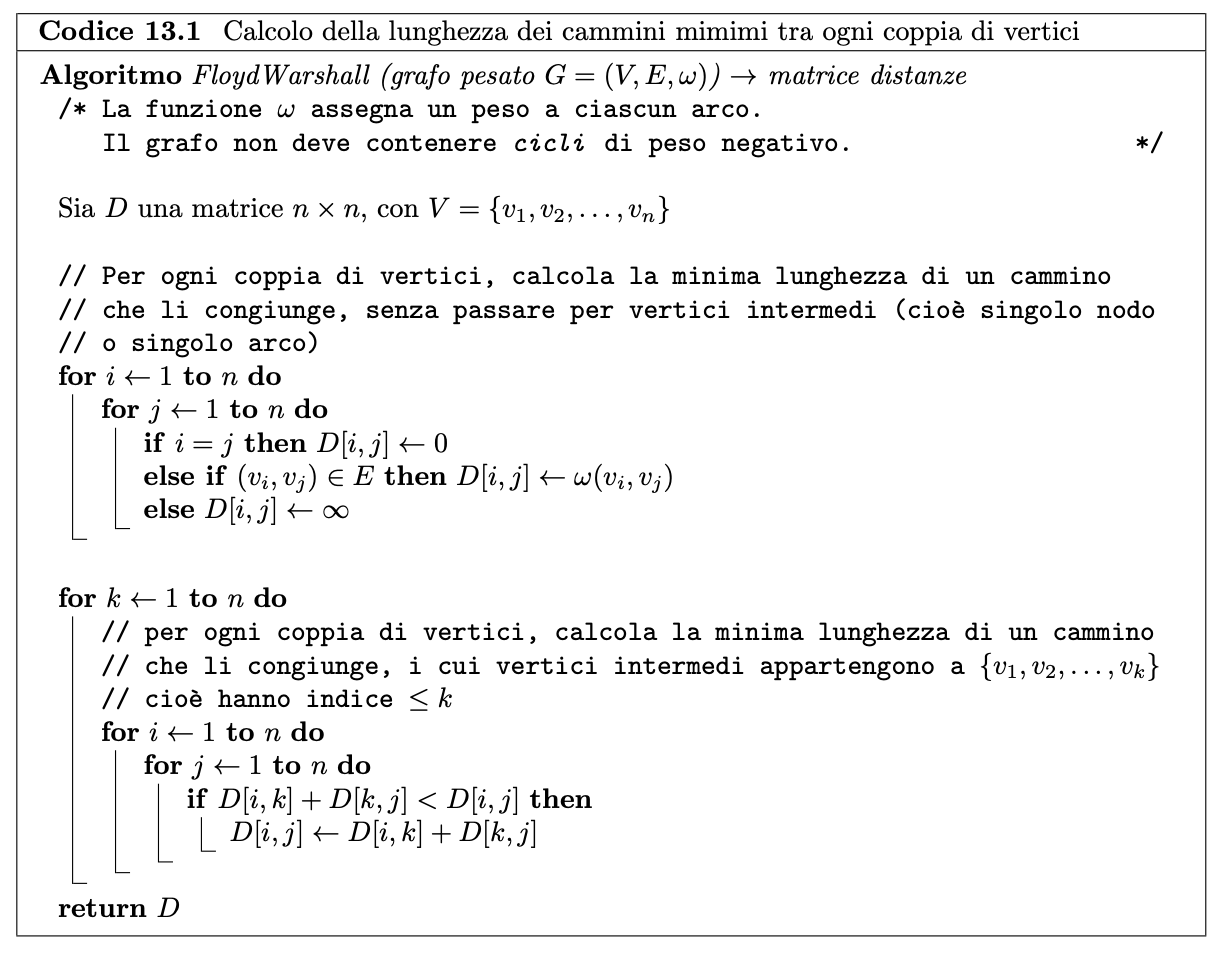
\includegraphics[scale=0.5]{floyd}
\end{center}
L'algoritmo lavora in tempo $T(n) = O(n^3)$

\subsection*{Algoritmo di Bellman \& Ford}
L’algoritmo di Bellman-Ford (1958-1962) consente la presenza di archi di peso negativo (ma non cicli negativi) e procede alla riduzione sistematica della stima della distanza minima calcolata per ciascun vertice.
\begin{center}
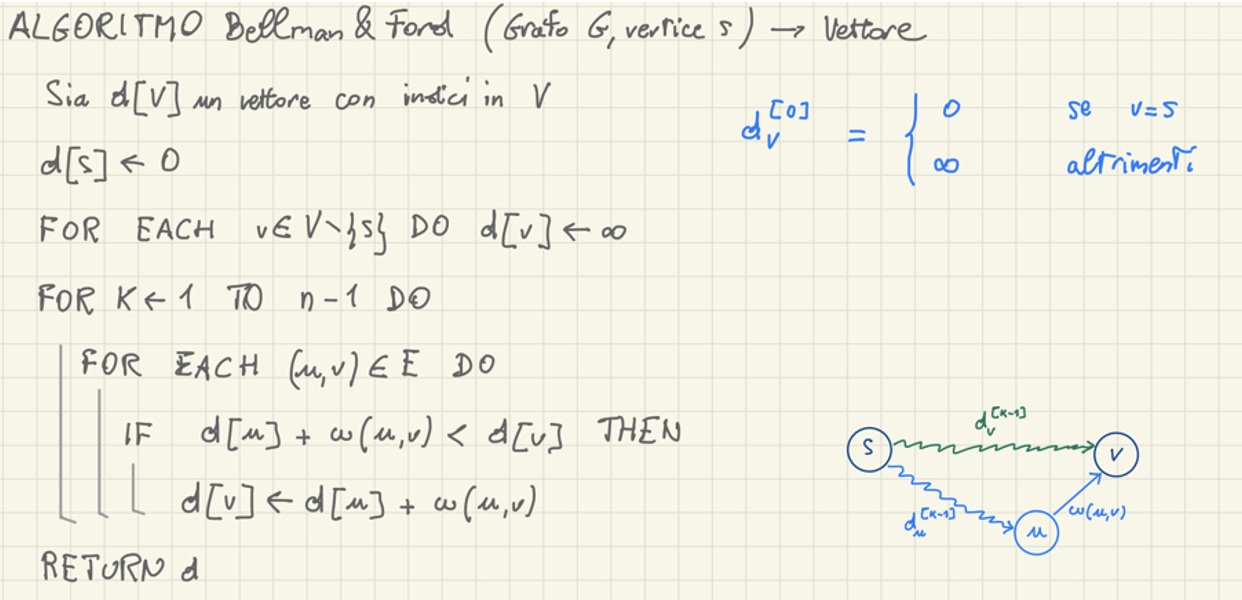
\includegraphics[scale=0.6]{bellman}
\end{center}
Ad ogni vertice viene assegnato un valore iniziale $\infty$, che viene aggiornato man mano partendo dal vertice iniziale. Una volta completato l'aggiornamento di tutti gli archi uscenti si passa al prosismo vertice, se la somma del valore è $<$ il valore $d_v$ è aggiornato, altrimenti $d_v$ è scartato\\
L'algoritmo lavora in tempo $T(n) = O(m*n)$


\subsection*{Algoritmo di Dijkstra}
L'algoritmo di Dijkstra è più efficiente di quello di Bellman-Ford, ma si applica solo a grafi privi di archi di peso negativo basato sulla strategia greedy. \begin{itemize}
\item Inizialmente tutti i $d_v$ che non sono il vertice iniziale hanno un valore assegnato a $\infty$, 0 se invece solo il vertice iniziale; viene creato $C$ insieme di vertici candidati inizialmente $C= V$
\item preleva da $C$ un vertice $u$ con $d_u$ minima
\item $d_u$ diventa definita e aggiorna $d[v]$ per ogni $v$ adiacente a $u$
\end{itemize}
\begin{center}
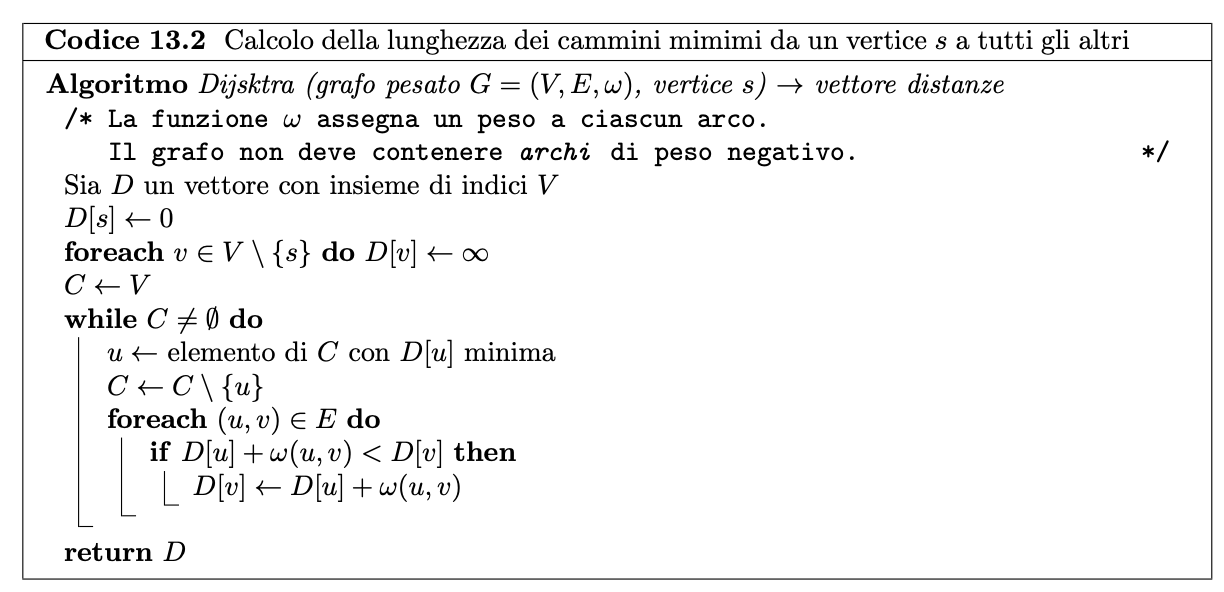
\includegraphics[scale=0.6]{dijkstra}
\end{center}
L'algoritmo lavora in tempo $T(n) = O(m + nlongn)$


\section*{Hash e tabelle hash}
Vediamo prima di tutto una tabella riassuntiva dei tempi richiesti delle 3 operazioni nelle varie strutture che abbiamo affrontato:
\begin{center}
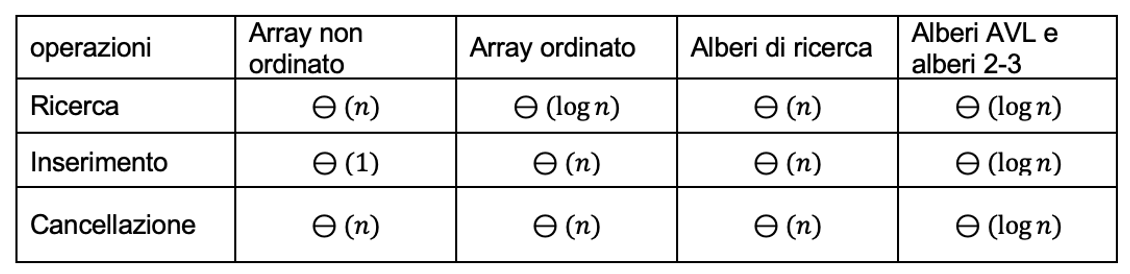
\includegraphics[scale=0.6]{h1}
\end{center}
Esiste tuttavia una struttura dati che inserisce in disordine i dati di proposito, in particolare le tabelle hash.\begin{itemize}
\item sia U = l'universo delle chiavi
\item sia {0, ... n-1} lo spazio delle chiavi
\end{itemize}
Una funzione di hash è una funzione che associa un elemento della chiave ad ogni elemento edgli indici così definita:
\begin{center}
$h = U \rightarrow{0, ... ,n-1}$
\end{center}
Una funzione di hash è perfetta se è iniettiva, ovvero se $u = v$, $h(u) != h(v)$, più una funzione di hash sparpaglia gli elementi, meglio è. E' tuttavia possibile che due elementi abbiamo una stessa chiave, in questo caso parliamo di $collisione$. 
Per gestire le collisioni possiamo adottare
\begin{itemize}
\item Strategie interne, ove le collisioni vengono gestite all’interno delle tabelle
\item Strategie esterne, ove collisioni vengono gestite esternamente dalle tabelle.\\
Viene impiegata una cosiddetta lista di collisioni, all’inserimento di un elemento, essa non viene inserita nella tabella, ma viene collegata alla lettera corretta, ne consegue che la tabella deve essere dimensionata in maniera corretta da permettere il contenimento di tutte le chiavi.
\end{itemize}
\begin{center}
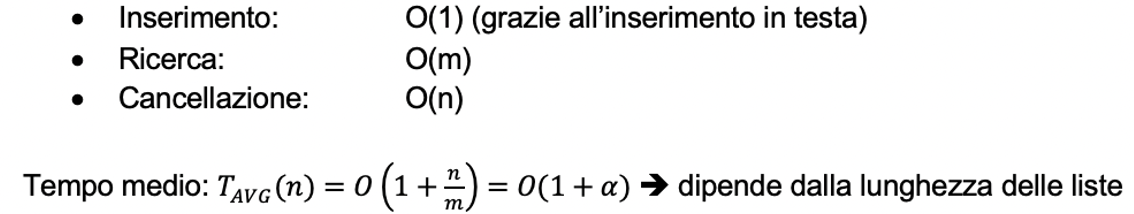
\includegraphics[scale=0.6]{h2}
\end{center}
\subsection*{Problema di agglomerazione primaria}
Il problema di agglomerazione primaria si presenta quando abbiamo una zona in cui si concentrano molti dati. Questo succede quando la funzione di hashing non sparpaglia sufficientemente bene. Consideriamo un esempio pratico:
\begin{itemize}
\item sia $U = stringhe di lettere$
\item sia $h(x) = ord(1°lettera$ $di$ $x)$\\
eg. $ord(A) =1$, $ord(Z) = 25$
\end{itemize}
Consideriamo la sequenza: Pippo, Paperino, Topolino, Qui, Pluto, Quo, Qua, Paperoga
\begin{center}
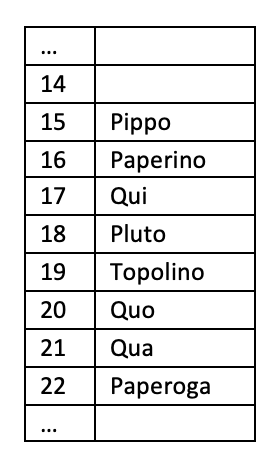
\includegraphics[scale=0.6]{h3}
\end{center}
Per aggirare questo problema, possiamo implementare l'indirizzamento aperto. L'indirizzamento aperto è basato su una funzione ausiliaria $c(k,i)$, ove $k = chiave$ e $i = intero$ con $i = 1,...n$ ordine della scansione.\\
Definiamo scansione lineare: \begin{center} $c(k,i) = (h(k)+i)$ $mod$ $m$\end{center}
e scansione quadratica:  \begin{center} $c(k,i) = [h(k)+c1i+ c2i^2]$ $mod$ $m$\end{center}
Questa funzione ausiliaria ci permette di aggirare il problema di agglomerazione primaria, ma non interviene sull'agglomerazione secondaria
\subsection*{Hashing doppio}
L'hashing doppio è applicabile quando all'inserimento di un valore nella tabella di hash, troviamo un posto occupato. In questo caso possiamo impiegare una seconda funzione di hashing, diversa.
Il problema con questa implementazione è che la cancellazione crea qualche problema, infatti ad ogni cancellazione, dovremmo ristrutturare tutta la tabella perché potremmo perdere i legami che legano le celle, che vengono utilizzati nelle ricerche.\\
Risolviamo tale problema introducendo un flag booleano di cancellazione, al momento della cancellazione effettuiamo solo una cancellazione virtuale, e non effettiva.
\subsection*{Rehashing}
Il rehashing avviene quando la tabella viene riempita oltre la soglia prestabilita. Viene creata una tabella più grande (di solito il doppio), in cui vengono trasferiti tutti gli elementi, per continuare l'hashing. In particolare dobbiamo andare a vedere la \emph{funzione hashing della nuova tabella, e il costo in termini di tempo}\\
\emph{La funzione hash}\\
Solitamente la funzione hash è parametrica rispetto alla dimensione $m$ della tabella, in particolare \begin{center}
$h_m(k) = f(k)$ $mod$ $m$
\end{center}
Ove $f(k)$ è un'altra funzione hash che restituisce un interno molto grande. Se $f$ è uniforme, allora anche $h_m$ è uniforme.
\section*{Complessità computazionale}
A partire da un problema possiamo effettuare analisi classificando stimando rispetto alle risorse necessarie e sufficienti per risolvere il problema. Dato un problema da risolvere cerchiamo un algoritmo risolutivo, e mentre lo facciamo facciamo anche la stima delle risorse utilizzate dallo specifico algoritmo, che possono essere spazio, tempo, numero di confronti, etc. \\
Quando parliamo di \emph{classe di complessità} facciamo riferimento all'insieme dei problemi che possono essere risolti utilizzando la stessa classe di quantità di una data risorsa.
\begin{center}
$r$ risorsa computazionale\\
$\pi$ problema risolvibile algoritmicamente
\end{center}
\emph{quanta risorsa r è necessaria e sufficiente per risolvere $\pi$?}
\subsection*{Classe P}
Identifichiamo quindi la classe $P$, ovvero la classe di problemi che possono essere risolti in tempo polinomiale rispetto alla lunghezza dell'output. In particolare questa classe è chiamata $PTIME$, ma non è l'unica, altre classi che ci interessano sono:
\begin{itemize}
\item PSPACE: classi di problemi che possono essere risolti in spazio polinomiale
\item EXPTIME: classi di rpoblemi che possono essere risolti in tempo esponenziale
\end{itemize}
Ne consegue che $P \subseteq EXPTIME$
\subsection*{Tipologie di problemi}
Consideriamo:
\begin{center}
I = universo delle possibili istanze di input\\
S = universo delle soluzioni\\
$\pi$ = universo dei problemi\\
\end{center}
Di norma i problemi che affrontiamo rientrano in 3 macro-categorie:
\begin{itemize}
\item Ricerca: dato $x\in I$, trovare $s \in S$ t.c. $(x,s)\in I$
\item Ottimizzazione: dato  $x\in I$, trovare $s \in S$ t.c. $(x,s)\in I$ che soddisfi un criterio di ottimalità fissato (ad esempio minimo o massimo)
\item Decisione: data un universo di soluzioni $S = {0,1}$:\\
$(x,1) \in \pi$ istanze positive ovvero $\pi(x) = 1$
$(x,0) \in \pi$ istanze negative ovvero $\pi(x) = 0$
\end{itemize}
Dato un problema di ottimizzazione possiamo passare ad un problema di decisione, ad esempio:
\begin{itemize}
\item Ottimizzazione: dato un grafo $G(V,E,\omega)$  trovare l’albero ricoprente minimo
\item Decisione: dato un grafo $G(V,E,\omega)$ con $K\in N$ esiste l’albero ricoprente di $G$ di peso $\leq K$?
\end{itemize}
\subsection*{Relazione spazio/tempo}
Consideriamo un tempo $t$ (ovvero con tempo fissato), ogni istruzione elementare visita al massimo $k$ celle di memoria. In particolare il numero di celle visitate (lo spazio) è limitato dal tempo $t$:
\begin{center}
$t \leq kt$
\end{center}
Possiamo quindi concludere che un tempo polinomiale implica uno spazio polinomiale:
\begin{center}
$P \subseteq PSPACE$
\end{center}
Consideriamo invece uno spazio $s$ (ovvero con spazio fissato), se consideriamo $s$ locazioni di memoria di $k$ bit ciascuno, abbiamo al massimo $2^k$ configurazioni diverse. Rispetto allo spazio abbiamo $2^{ks}$ configurazioni diverse dello spazio.
\begin{center}
$t \leq p2^{ks}$
\end{center}
Possiamo quindi concludere che uno spazio polinomiale implica un tempo al massimo esponenziale.
\begin{center}
$PSPACE \subseteq EXPTIME$
\end{center}
Possiamo infine concludere che:
\begin{center}
$P \subseteq PSPACE \subseteq EXPTIME$
\end{center}
Nessuno è riuscito a verificare che $P$ e $EXPTIME$ sono propri. Si sa tuttavia che almeno una delle due è propria. Sappiamo infatti che $P \subset EXPTIME$
\section*{Problemi difficili}
\subsection*{Problema Clique}
\begin{itemize}
\item Istanza: dato un grafo non orientato $G= (V,E)$ \\
ed un intero $k \geq 0$
\item Problema: esiste un sottografo completo di $G$ con $k$ vertici?
\end{itemize}
\subsection*{Problema delle formule booleane | soddisfacibilità SODD}
\begin{itemize}
\item Istanza: data una formula booleana $\phi$ in forma normale congiuntiva con un insieme di variabili $V$
\item Problema: esiste un assegnamento delle variabili in $V$ che rende vera $\phi$, ovvero
\item Una modalità per approcciare il problema sarebbe di verificare tutti i possibili assegnamenti di valori alle variabili $x_1, ..., x_n$
\begin{center}
$\phi(f) = 1$
\end{center}
\end{itemize}
\subsection*{Algoritmi non deterministici}
Un algoritmo non deterministico è un algoritmo che, anche per lo stesso input, può esibire comportamenti diversi su corse diverse. In altre parole, è un algoritmo in cui il risultato di ogni algoritmo non è definito in modo univoco e il risultato potrebbe essere casuale.
\subsection*{La classe NP}
La classe NP è la classe dei problemi di decisione risolvibili in tempo polinomiale da algoritmi non deterministici, oppure la classe dei problemi di decisione con certiciati verificabili in tempo polinomiale.
Gli algoritmi che risolvono problemi NP possono essere divisi in due fasi:
\begin{itemize}
\item fase non deterministica: che consiste nella costruzione del certificato
\item fase deterministica: che consiste nella fase di verifica del certificato in tempo polinomiale.
\end{itemize}
In particolare possiamo formalizzare che
\begin{center} $P \subseteq NP$\end{center}
Possiamo tuttavia dire che $P \neq NP$? Non lo sappiamo:
\begin{itemize}
\item in particolare se $P = NP$ ciò ci permettere di determinare se i problemi che possono essere verificati in tempo polinomiale possono essere anche risolti in tempo polinomiale
\item invece se $P \neq NP$ ciò ci permetterebbe di dire che problemi in NP sono più difficili da computare che da verificare, ovvero non possono essere risolti in tempo polinomiale, ma la risolta è verificabile in tempo polinomiale
\end{itemize}

\end{document}  